% Main document file for the Spin the Web Book
% This file orchestrates the entire book structure

\documentclass[11pt,openright,twoside,a4paper]{book}

% Load all packages and formatting
% Package imports for the Spin the Web Book
% This file contains all LaTeX package declarations

% Basic packages
\usepackage[utf8]{inputenc}
\usepackage[T1]{fontenc}
\usepackage[english]{babel}

% Page layout and geometry
\usepackage[a4paper,margin=2.5cm,inner=3cm,outer=2cm]{geometry}
\usepackage{fancyhdr}

% Typography and fonts
\usepackage{lmodern}
\usepackage{microtype}
\usepackage{setspace}
% Hybrid font setup: sans for headings, clear mono for code
\usepackage{tgheros} % TeX Gyre Heros (Helvetica-like) for sans headings
\usepackage[scaled=0.95]{inconsolata} % Inconsolata for code/listings

% Graphics and figures
\usepackage{graphicx}
\usepackage{float}
\usepackage{wrapfig}
\usepackage{subcaption}

% Tables
\usepackage{booktabs}
\usepackage{tabularx}
\usepackage{longtable}
\usepackage{array}

% Colors and highlighting
\usepackage{xcolor}
\usepackage{soul}

% Code listings and syntax highlighting
\usepackage{listings}

% Math and symbols
\usepackage{amsmath}
\usepackage{amssymb}
\usepackage{amsfonts}

% Cross-references and links
% Consolidated hyperref options here; metadata is set in formatting.tex
\usepackage[
  pdfusetitle,
  colorlinks=true,
  linkcolor=blue,
  filecolor=magenta,
  urlcolor=cyan,
  citecolor=green,
  bookmarks=true,
  bookmarksopen=true,
  bookmarksopenlevel=2
]{hyperref}
\usepackage{cleveref}
\usepackage{url}

% Special boxes and frames
\usepackage{tcolorbox}
\usepackage{framed}
\usepackage{mdframed}

% Index and glossary
\usepackage{makeidx}
% Glossaries: ensure entries hyperlink correctly and appear as a chapter in book class
\usepackage[acronym,toc,section=chapter,hyperfirst=true]{glossaries}

% Bibliography
\usepackage{natbib}

% Space handling for custom commands
\usepackage{xspace}

% Title page customization
\usepackage{titling}

% TikZ for diagrams
\usepackage{tikz}
\usetikzlibrary{shapes,arrows,positioning,fit,backgrounds,calc}

% Additional useful packages
\usepackage{enumitem}
\usepackage{multicol}
\usepackage{pdfpages}
\usepackage{afterpage}
\usepackage{placeins}

% Watermark (can be toggled by commenting out these lines)
\usepackage[firstpage=false]{draftwatermark}
\SetWatermarkText{WIP}
\SetWatermarkScale{0.7}
\SetWatermarkAngle{45}
\SetWatermarkColor[gray]{0.95}

% Package configurations
\tcbuselibrary{most}
\usepackage{datetime2}

% Formatting definitions for the Spin the Web Book
% This file contains all formatting and style definitions

% Hyperlink setup
\hypersetup{
    colorlinks=true,
    linkcolor=blue,
    filecolor=magenta,      
    urlcolor=cyan,
    citecolor=green,
    pdftitle={Spin the Web},
    pdfauthor={Giancarlo Trevisan (\organization)},
    pdfsubject={Enterprise Web Portal Development},
    pdfkeywords={WBDL, Web Spinner, Web Portal, Enterprise Software Integrator, STW},
    bookmarks=true,
    bookmarksopen=true,
    bookmarksopenlevel=2
}

% Page headers and footers
\pagestyle{fancy}
\fancyhf{}
\fancyhead[LE,RO]{\thepage}
\fancyhead[LO]{\nouppercase{\rightmark}}
\fancyhead[RE]{\nouppercase{\leftmark}}
\renewcommand{\headrulewidth}{0.4pt}
\renewcommand{\footrulewidth}{0pt}

% Fix header height warning
\setlength{\headheight}{14pt}

% Chapter and section formatting
\usepackage{titlesec}
\titleformat{\chapter}[display]
    {\sffamily\bfseries\huge}{\chaptertitlename\ \thechapter}{18pt}{\sffamily\bfseries\Huge}
% Tighter chapter spacing: before=36pt, after=24pt
\titlespacing*{\chapter}{0pt}{36pt}{24pt}

% Sans-serif for section levels
\titleformat{\section}
    {\Needspace{4\baselineskip}\sffamily\bfseries\Large}{\thesection~}{0pt}{}
% Tighter spacing around section headings
\titlespacing*{\section}{0pt}{1.5ex plus .5ex minus .2ex}{1.0ex plus .2ex}
\titleformat{\subsection}
    {\Needspace{3\baselineskip}\sffamily\bfseries\large}{\thesubsection~}{0pt}{}
\titlespacing*{\subsection}{0pt}{1.25ex plus .5ex minus .2ex}{0.8ex plus .2ex}
\titleformat{\subsubsection}
    {\Needspace{3\baselineskip}\sffamily\bfseries\normalsize}{\thesubsubsection~}{0pt}{}
\titlespacing*{\subsubsection}{0pt}{1.0ex plus .3ex minus .2ex}{0.6ex plus .1ex}

% Line spacing
\onehalfspacing

% Paragraph formatting
\setlength{\parindent}{0pt}
\setlength{\parskip}{0.5em}

% Avoid widows and orphans (single lines at page breaks)
\clubpenalty=10000
\widowpenalty=10000
\displaywidowpenalty=10000

% Also disallow page breaks that would leave only 1–2 lines
% at the top (clubs) or bottom (widows) of a page (e-TeX primitives)
\clubpenalties 2 10000 10000
\widowpenalties 2 10000 10000

% Allow more flexibility in line breaking and page height to reduce sparse pages
\raggedbottom
\tolerance=2000
\setlength{\emergencystretch}{3em}

% Ensure microtype features that help compaction are active
\microtypesetup{protrusion=true,expansion=true}

% Float placement tuning to better fill pages
\setcounter{topnumber}{3}
\setcounter{bottomnumber}{2}
\setcounter{totalnumber}{4}
\renewcommand{\topfraction}{0.9}
\renewcommand{\bottomfraction}{0.8}
\renewcommand{\textfraction}{0.07}
\renewcommand{\floatpagefraction}{0.8}

% List formatting
\setlist{nosep}
\setlist[itemize]{leftmargin=1.5em}
\setlist[enumerate]{leftmargin=1.5em}

% Code listing colors and styles
\definecolor{codebackground}{RGB}{248,248,248}
\definecolor{codeborder}{RGB}{255,255,255}
\definecolor{commentcolor}{RGB}{106,153,85}
\definecolor{keywordcolor}{RGB}{86,156,214}
\definecolor{stringcolor}{RGB}{206,145,120}

% Listings configuration
% Enable UTF-8 characters commonly used in examples inside listings
\lstset{
        inputencoding=utf8,
        literate=
            {‹}{{\guilsinglleft}}1 {›}{{\guilsinglright}}1 % single guillemets
            {«}{{\guillemotleft}}1 {»}{{\guillemotright}}1 % double guillemets
            {“}{{\textquotedblleft}}1 {”}{{\textquotedblright}}1 % curly double quotes
            {‘}{{\textquoteleft}}1 {’}{{\textquoteright}}1 % curly single quotes/apostrophe
            {–}{{\textendash}}1 {—}{{\textemdash}}1 % en/em dashes
            {…}{{\ldots}}1 % ellipsis
            {°}{{\textdegree}}1 % degree symbol
            {€}{{\texteuro}}1 % euro sign
            {™}{{\texttrademark}}1 {®}{{\textregistered}}1 {©}{{\textcopyright}}1 % symbols
            {•}{{\textbullet}}1
}

% Define JavaScript language if not provided by listings on this TeX distro
% (Some MiKTeX setups lack JavaScript by default.)
\lstdefinelanguage{JavaScript}{
    morekeywords={break,case,catch,continue,debugger,default,delete,do,else,finally,for,function,if,in,instanceof,new,return,switch,this,throw,try,typeof,var,void,while,with,const,let,of,import,from,export,class,extends,super,static,yield,await,async,true,false,null,undefined},
    sensitive=true,
    morecomment=[l]{//},
    morecomment=[s]{/*}{*/},
    morestring=[b]',
    morestring=[b]",
}

% Define JSON language (based on JavaScript, strings highlighted)
\lstdefinelanguage{JSON}{
    basicstyle=\ttfamily\small,
    showstringspaces=false,
    morestring=[b]",
    stringstyle=\color{stringcolor},
    morecomment=[l]{//},
}

% Define JSON language style for listings
\lstdefinestyle{jsonstyle}{
    language=JavaScript, % Use JavaScript as a base for syntax
    morestring=[b]",
    stringstyle=\color{stringcolor},
    morekeywords={true,false,null,_id,type,name,slug,keywords,description,visibility,children,mainpage,langs,datasources,version,namespace,rules,role,visible,subtype,query,layout,options,connectionString,baseUrl},
    keywordstyle=\color{keywordcolor},
    showstringspaces=false,
    basicstyle=\ttfamily\small,
    upquote=true,
    tabsize=2,
    breaklines=true,
    breakatwhitespace=true,
    frame=single,
    backgroundcolor=\color{codebackground},
    rulecolor=\color{codeborder},
}

% Define WBLL language for listings (custom DSL used in this book)
% Highlights tokens (single-letter mnemonics), supports comments and single-quoted strings
\lstdefinelanguage{WBLL}{
    morekeywords={t,e,f,r,l,w,m,h},
    sensitive=true,
    morecomment=[l]{//},
    morecomment=[s]{/*}{*/},
    morestring=[b]',
}

% Optional: a compact style for inline WBLL code blocks
\lstdefinestyle{wball}{
    language=WBLL,
    basicstyle=\ttfamily\small,
    showstringspaces=false,
    upquote=true,
}

% Custom boxes for examples, notes, warnings
\newtcolorbox{examplebox}[1][]{
    colback=blue!5!white,
    colframe=blue!75!black,
    title=Example,
    #1
}

\newtcolorbox{notebox}[1][]{
    colback=green!5!white,
    colframe=green!75!black,
    title=Note,
    #1
}

\newtcolorbox{warningbox}[1][]{
    colback=red!5!white,
    colframe=red!75!black,
    title=Warning,
    #1
}

\newtcolorbox{tipbox}[1][]{
    colback=orange!5!white,
    colframe=orange!75!black,
    title=Tip,
    #1
}

% Figure and table captions
\usepackage{caption}
\captionsetup{
    font=small,
    labelfont=bf,
    format=hang,
    indention=0cm,
    margin=1cm
}

% Glossary style
\setglossarystyle{altlist}

\usepackage{upquote}

\lstset{
  upquote=true,
  showstringspaces=false,
  keepspaces=true,
  columns=fullflexible,
  % normalize curly quotes to straight quotes in listings
    literate={’}{{'}}1 {‘}{{'}}1 {“}{{"}}1 {”}{{"}}1 {€}{{\texteuro}}1
}

\lstset{
    frame=single,                % Draw a box around listings
    breaklines=true,             % Enable automatic line breaking
    breakatwhitespace=true,      % Prefer breaking at whitespace
    postbreak=\mbox{\textcolor{red}{$\hookrightarrow$}\space}, % Mark wrapped lines
    basicstyle=\ttfamily\small,  % Monospaced font, small size
    backgroundcolor=\color{codebackground},
    rulecolor=\color{codeborder},
    showstringspaces=false,
    tabsize=2,
    xleftmargin=1em,
    xrightmargin=1em,
    aboveskip=1em,
    belowskip=1em,
    captionpos=b
}

% Custom commands for the Spin the Web Book
% This file contains custom LaTeX commands and macros

% Define subtitle command
\makeatletter
\newcommand{\subtitle}[1]{\gdef\@subtitle{#1}}
\newcommand{\@subtitle}{}
\makeatother

% Project-specific terminology commands
% Organization macro
\newcommand{\organization}{Spin the Web Foundation}

% Project-specific terminology commands
\newcommand{\wbdl}{\texttt{WBDL}\xspace}
\newcommand{\wbpl}{\texttt{WBPL}\xspace}
\newcommand{\wbll}{\texttt{WBLL}\xspace}
\newcommand{\webspinner}{\textit{Web Spinner}\xspace}
\newcommand{\webbase}{\textit{webbase}\xspace}
\newcommand{\webbaselet}{\textit{webbaselet}\xspace}
\newcommand{\webbaselets}{\textit{webbaselets}\xspace}
\newcommand{\studio}{\textit{Spin the Web Studio}\xspace}

% Acronyms for enterprise systems
\newcommand{\erp}{\texttt{ERP}\xspace}
\newcommand{\crm}{\texttt{CRM}\xspace}
\newcommand{\bpms}{\texttt{BPMS}\xspace}
\newcommand{\mrp}{\texttt{MRP}\xspace}
\newcommand{\rest}{\texttt{REST}\xspace}

% WBDL element types
\newcommand{\stwsite}{\texttt{STWSite}\xspace}
\newcommand{\stwarea}{\texttt{STWArea}\xspace}
\newcommand{\stwpage}{\texttt{STWPage}\xspace}
\newcommand{\stwcontent}{\texttt{STWContent}\xspace}
\newcommand{\stwele}{\texttt{STWElement}\xspace}
\newcommand{\stwvis}{\texttt{STWVisibility}\xspace}
\newcommand{\stwloc}{\texttt{STWLocalized}\xspace}

% Code and file references
\newcommand{\codefile}[1]{\texttt{#1}\xspace}
\newcommand{\jsonfld}[1]{\texttt{"#1"}\xspace}

% Commands for JSON Schema
\newcommand{\jsontype}[1]{\texttt{#1}\xspace}
\newcommand{\jsonprop}[1]{\texttt{#1}\xspace}

% Figure and table reference commands
\newcommand{\figref}[1]{Figure~\ref{#1}}
\newcommand{\tabref}[1]{Table~\ref{#1}}
\newcommand{\chapref}[1]{Chapter~\ref{#1}}
\newcommand{\secref}[1]{Section~\ref{#1}}

% Math notation for technical concepts
\newcommand{\set}[1]{\{#1\}}
\newcommand{\tuple}[1]{\langle#1\rangle}

% Special formatting for version numbers
\newcommand{\version}[1]{\texttt{v#1}\xspace}

% Index entries for consistent indexing
\newcommand{\indexwbdl}{\index{WBDL|textbf}}
\newcommand{\indexwbpl}{\index{WBPL|textbf}}
\newcommand{\indexwbll}{\index{WBLL|textbf}}
\newcommand{\indexspinner}{\index{Web Spinner|textbf}}
\newcommand{\indexstudio}{\index{Spin the Web Studio|textbf}}

% Glossary entries (to be defined in glossary file)
\newcommand{\glswebbase}{\gls{webbase}}
\newcommand{\glswebbaselet}{\gls{webbaselet}}
\newcommand{\glsportal}{\gls{portal}}

% Commands for consistent cross-referencing
\newcommand{\xref}[2]{\hyperref[#1]{#2}}


% Document metadata
\title{Spin the Web}
\subtitle{Weaving the Future of Digital Portals}
\author{Giancarlo Trevisan}
\date{\today}

% Generate index
\makeindex
\makeglossaries

\begin{document}

%% FRONT MATTER %%
\frontmatter
% Title page for the Spin the Web Book
\begin{titlepage}
\centering

% Logo or graphic
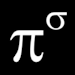
\includegraphics[width=0.15\textwidth]{figures/logo-bn_75x75.png}\\[1cm]

\vspace*{1cm}

% Title
\makeatletter
{\Huge\bfseries \@title\\[0.5cm]}

% Subtitle (if defined)
\ifx\@subtitle\@empty\else
{\Large \@subtitle\\[1.5cm]}
\fi

% Author
{\large\textsc{\@author}\\[2cm]}

% Version and date
{\large Version 1.0\\[0.5cm]}
{\large \@date\\[2cm]}
\makeatother

\vfill

% Publisher or organization
{\large KeyVisions di Giancarlo Trevisan\\[0.5cm]}

% Abstract or tagline
\begin{quote}
\centering
\textit{A comprehensive guide to building unified, role-based web portals that serve as virtualized companies, integrating disparate enterprise systems into coherent digital channels.}
\end{quote}

\end{titlepage}

% Copyright page
\thispagestyle{empty}
\null\vfill
\noindent
% Copyright page
\thispagestyle{empty}
\vspace*{\fill}
\begin{center}
\small
Copyright \copyright\ \the\year\ Giancarlo Trevisan. All rights reserved.

\medskip

\noindent
No part of this publication may be reproduced, distributed, or transmitted in any form or by any means, including photocopying, recording, or other electronic or mechanical methods, without the prior written permission of the author, except in the case of brief quotations embodied in critical reviews and certain other noncommercial uses permitted by copyright law.

\medskip

\noindent
\textbf{First Edition}

\medskip

\noindent
For more information about the Spin the Web Project, visit: \\
\url{https://www.spintheweb.org}

\medskip

\noindent
ISBN: [To be assigned]
\end{center}

\clearpage

% License page for the book
\cleardoublepage
\thispagestyle{empty}
\begin{center}
{\Large License}\\[1.25em]
Copyright \textcopyright{} 2025 Giancarlo Trevisan\\[0.75em]
This work is licensed under the\\
{\bfseries Creative Commons Attribution--ShareAlike 4.0 International}\\
(CC BY--SA 4.0).\\[0.75em]
To view a copy of this license, visit\\
\url{https://creativecommons.org/licenses/by-sa/4.0/}
\end{center}

\vfill
\noindent You are free to share and adapt the material for any purpose, even commercially, provided that you give appropriate credit and distribute your contributions under the same license as the original.

% Abstract for the Spin the Web Book

\chapter*{Abstract}
\addcontentsline{toc}{chapter}{Abstract}
\textbf{Spin the Web} is an open source framework for building enterprise web portals (``portals'') with the intent of virtualizing the enterprise brand—\textit{eBranding}. It addresses the persistent challenge of unifying heterogeneous enterprise systems (ERP, CRM, BPMS, and MRP systems) behind a single, role-aware digital channel, providing consistent abstractions over disparate backends. The framework is stewarded by the Spin the Web Foundation.

The framework comprises three core components:
\begin{enumerate}
\item \textbf{Webbase Description Language (WBDL)}: A declarative language for modeling portal structure, content, and behavior.
\item \textbf{Web Spinner}: An engine that interprets webbases (modular portal definitions written in WBDL) to dynamically generate personalized user experiences with real-time content delivery and role-based authorization.
\item \textbf{Spin the Web Studio}: An authoring webbaselet for in-place editing of webbases; it also serves as a laboratory for exercising the Web Spinner.
\end{enumerate}

The project also introduces:
\begin{itemize}
\item \textbf{Webbaselets}: Modular, self-contained WBDL fragments that encapsulate integrations with enterprise systems.
\item \textbf{Webbase Placeholders Language (WBPL)}: A security-conscious templating mechanism for parameterized queries.
\item \textbf{Webbase Layout Language (WBLL)}: A token-based templating language for presentation and rendering.
\item \textbf{Virtualized Company paradigm}: A unified portal interface for customers, employees, suppliers, partners, and governance stakeholders, with the primary objective of digitally harboring the brand (\textit{eBranding}).
\end{itemize}

This book combines foundational concepts with practical guidance for developers, integrators, and technology leaders seeking to modernize digital channels.

\textbf{Keywords:} web portals; eBranding; webbase; webbaselets; framework; Spin the Web Foundation; STW.

\clearpage

% Preface for the Spin the Web Book

\chapter*{Preface}
\addcontentsline{toc}{chapter}{Preface}

\section*{Why This Book Exists}

In the rapidly evolving landscape of enterprise software, organizations find themselves trapped in a web of disparate systems, each with its own interface, data model, and user experience paradigm. Employees struggle to navigate between multiple applications, customers face fragmented touchpoints, and partners encounter inconsistent integration patterns. The promise of digital transformation often falls short because these systems remain fundamentally siloed.

Spin the Web emerged from real-world frustration with this fragmentation. After years of building custom integrations, developing multiple user interfaces, and watching organizations struggle with the complexity of their own digital ecosystems, it became clear that a fundamentally different approach was needed.

\section*{What Makes This Different}

This book introduces a paradigm shift: instead of trying to integrate disparate systems at the data level, we integrate them at the experience level. The \wbdl specification provides a unified way to describe portal structures that can encompass any type of enterprise system. The \webspinner engine handles the complex task of real-time personalization and content delivery. The \studio provides the tools needed to build and maintain these portals efficiently.

What sets this approach apart is the concept of the "virtualized company"—a single, coherent digital interface that adapts to each user's role and needs, whether they are a customer, employee, supplier, or partner. This isn't just another portal framework; it's a complete rethinking of how organizations should present themselves digitally.

\section*{The Mathematical Philosophy}

The Spin the Web logo incorporates the symbols $\pi$ (pi) and $\sigma$ (sigma), which together represent circular variance—a statistical measure of how data points deviate from a circular mean. This mathematical concept serves as the foundational heuristic for the entire project.

In traditional enterprise environments, user experiences exhibit high variance: different interfaces, inconsistent workflows, and disparate data presentations create friction and confusion. Each system operates independently, leading to significant "deviation" from an optimal user experience pattern.

Spin the Web applies the principle of minimizing circular variance to enterprise portal design. Just as circular variance measures deviation from an ideal circular pattern, our framework aims to reduce the experiential variance that users encounter when interacting with complex enterprise systems.

This manifests in several key ways:
\begin{itemize}
\item \textbf{Cyclical Integration}: Rather than linear system-to-system integration, the framework creates circular workflows that naturally return users to a central hub
\item \textbf{Variance Minimization}: The \wbdl specification standardizes how different enterprise systems present themselves, reducing interface variance
\item \textbf{Harmonic Convergence}: Multiple stakeholder needs converge on a single, adaptable interface that minimizes deviation from each user's optimal experience
\item \textbf{Mathematical Precision}: The framework applies systematic, measurable approaches to reducing complexity rather than ad-hoc solutions
\end{itemize}

Like a spider's web, which exhibits mathematical precision in its radial structure, the Spin the Web architecture creates optimal pathways with minimal variance from the ideal pattern. This mathematical foundation ensures that the framework scales efficiently while maintaining coherent user experiences across diverse enterprise environments.

\section*{Who Should Read This Book}

This book is written for professional software developers, enterprise architects, and technology leaders who are responsible for building or maintaining complex web-based systems. While the concepts are accessible to developers with basic web development experience, the focus is on enterprise-grade solutions that require sophisticated understanding of system integration, security, and scalability.

Specifically, this book will be valuable to:
\begin{itemize}
\item Full-stack developers building enterprise web applications
\item System architects designing portal solutions
\item Development team leads planning integration strategies
\item Technology consultants working with enterprise clients
\item CIOs and CTOs evaluating portal technologies
\end{itemize}

\section*{How This Book Is Organized}

The book follows a logical progression from concepts to implementation:

\textbf{Parts I-II} establish the theoretical foundations, explaining the problem space and introducing the core concepts of Spin the Web.

\textbf{Parts III-V} dive deep into the three technical pillars: the \wbdl language specification, the \webspinner engine architecture, and the \studio development environment.

\textbf{Parts VI-VII} focus on practical implementation, covering installation, configuration, security, and operational concerns.

\textbf{Part VIII} explores advanced topics and future directions, including AI integration and enterprise-scale deployment patterns.

Each part builds upon previous concepts while remaining sufficiently self-contained for reference use.

\section*{Acknowledgments}

This work builds upon decades of innovation in web technologies, enterprise software architecture, and user experience design. Special recognition goes to the communities behind XML Schema, JSON Schema, and the countless open-source projects that make modern web development possible.

The practical insights in this book were refined through collaboration with enterprise development teams, integration partners, and the broader community of developers working to solve real-world portal challenges.

\section*{Feedback and Evolution}

Spin the Web continues to evolve based on real-world usage and community feedback. Readers are encouraged to share their experiences, suggest improvements, and contribute to the ongoing development of the framework.

For updates, additional resources, and community discussions, visit \url{https://www.spintheweb.org}.

\vspace{1cm}
\hfill Giancarlo Trevisan \\
\hfill \today

\clearpage


% Table of contents
\tableofcontents

%% MAIN MATTER %%
\mainmatter

% Part I: Foundations and Concepts
\part{Foundations and Concepts}
% Part I: Foundations and Concepts

\chapter*{Introduction to Part I}
\addcontentsline{toc}{chapter}{Introduction to Part I}
\label{part:foundations}

\begin{quote}
\textit{"The best way to predict the future is to create it."} \\
— Peter Drucker
\end{quote}

In this opening part, we explore the historical origins and fundamental challenges that led to the Spin the Web Project, and introduce the conceptual foundations that guide its approach to enterprise portal development.

We begin with the project's genesis in the late 1990s, tracing its evolution from a practical business challenge to a comprehensive framework. We then examine the current landscape of enterprise software, where organizations struggle with fragmented user experiences across multiple systems. Next, we introduce the revolutionary concept of the "virtualized company"—a unified digital interface that adapts to each stakeholder's role and needs.

Finally, we provide a comprehensive overview of the three-pillar architecture that makes this vision possible: the \wbdl{} specification for describing portal structures, the \webspinner{} engine for dynamic content delivery, and the \studio{} for development and maintenance.

\begin{description}
\item[\textbf{Chapter 0: Project Genesis and Historical Context}] (\cref{chap:genesis}) -- Explores the real-world origins of the Spin the Web Project, from its birth in an Italian jewelry business in the late 1990s through the evolution of the eBranding concept. This chapter provides crucial context for understanding both the technical innovations and business philosophy underlying the framework.

\item[\textbf{Chapter 1: Introduction to Enterprise Portal Challenges}] (\cref{chap:intro}) -- Examines the contemporary challenges facing modern enterprises in their digital transformation journeys and introduces the foundational concepts of the Spin the Web Project.

\item[\textbf{Chapter 2: Web Spinner Architecture and Mechanics}] (\cref{chap:virtualized}) -- Provides a comprehensive overview of the Web Spinner engine, detailing its architecture, mechanics, and operational patterns for dynamic portal generation.

\item[\textbf{Chapter 3: Three-Pillar Architecture Overview}] (\cref{chap:architecture}) -- Introduces the complete framework architecture and the relationships between \wbdl{}, the \webspinner{}, and the \studio{}.

\item[\textbf{Chapter 4: Learning from Experience}] (\cref{chap:learning}) -- Explores the patterns, insights, and methodologies that have emerged from years of portal development, providing the experiential foundation for understanding the systematic approach embodied in the Spin the Web Project.
\end{description}

These foundational concepts will prepare you for the detailed technical exploration that follows in subsequent parts of the book.

% Chapter 1: Project Genesis and Historical Context
\chapter{Project Genesis and Historical Context}
\label{chap:genesis}

This chapter explores the real-world origins of Spin the Web, tracing its evolution from a practical business challenge in the late 1990s to the systematic framework presented in this book. Understanding this genesis provides crucial context for appreciating both the technical innovations and the business philosophy that underpin the project.

\section{The Italian Jewelry Business Challenge}

In the late 1990s, the digital landscape was vastly different from today's interconnected world. Enterprise software was fragmented, web technologies were in their infancy, and businesses struggled to integrate their complex operational structures into cohesive digital experiences.

It was during this period that the seeds of Spin the Web were planted through a consulting engagement with an Italian jewelry business. This company represented the complexity typical of many enterprises: a nationwide sales force, distributed points of sale, international suppliers, in-house and national jewelry designers and manufacturers, a help desk, and a call center. Each component of this business ecosystem had its own requirements, processes, and stakeholders.

The challenge was clear: how to network this intricate structure in a way that would enable seamless collaboration, efficient information flow, and unified business processes across all participants in the ecosystem.

\section{From Lotus Notes to Web Technologies}

\subsection{The Lotus Notes Solution}

To address their networking needs, the company's IT department had implemented \textbf{Lotus Notes}, a collaborative client-server software platform developed at IBM. This choice was both sensible and forward-thinking for its time:

\begin{itemize}
\item \textbf{Effective Use of Available Connectivity}: Lotus Notes made intelligent use of the limited connectivity options available in the late 1990s
\item \textbf{Data Replication}: The platform successfully replicated data stored in a proprietary NoSQL database across distributed locations
\item \textbf{Development Environment}: It provided a respectable development environment for building front-ends to interact with business data
\item \textbf{Collaborative Features}: Beyond data management, Notes offered collaborative features that enhanced team communication
\item \textbf{Multi-Purpose Platform}: The sales force and points of sale used it to browse product catalogs and place orders, while the help desk and call center leveraged it as a knowledge base
\end{itemize}

\subsection{The Hybrid Solution Challenge}

When tasked with developing a solution to interface with the manufacturers, a significant technical challenge emerged. Lotus Notes did not handle SQL data particularly well, creating a mismatch between the platform's strengths and the manufacturers' data systems.

The solution adopted was a hybrid approach—a compromise that bridged the gap between the Notes environment and SQL-based manufacturing systems. While this approach was functional and met the immediate business needs, it highlighted a fundamental limitation: the difficulty of creating truly unified interfaces when working with disparate systems and technologies.

This experience planted the first seeds of what would later become the \webbaselet{} concept—the idea that different business systems could be unified through a common interface layer without requiring them to abandon their underlying architectures.

\section{The Dynamic Web Pages Revelation}

\subsection{The Internet Evolution}

As this project unfolded, the Internet was undergoing a revolutionary transformation. Dynamic web pages were making their debut\footnote{The technologies primarily referenced are ASP and PHP, which made dynamic pages easier to build. CGI had been available for some time and could accomplish similar functionality, but these newer technologies significantly lowered the barrier to entry.}, fundamentally changing how web applications could be conceived and implemented.

A dynamic web page represented a paradigm shift: rather than serving static HTML content, web servers could now assemble pages on-demand in response to specific client requests. This concept proved to be profoundly powerful and opened up entirely new possibilities for enterprise applications.

\subsection{The Conceptual Breakthrough}

The revelation came through understanding the full implications of dynamic page generation:

\begin{itemize}
\item \textbf{Universal Data Access}: Data sources in general could be queried by the web server in response to client requests
\item \textbf{On-Demand Rendering}: Fetched data could be rendered as HTML before being sent to the client
\item \textbf{Intuitive Data Interaction}: Clients could inspect data intuitively and perform insertions, updates, and deletions (CRUD operations)
\item \textbf{Unified Interface}: The same web page could host data coming from disparate data sources in a coherent, tailored graphical user interface
\end{itemize}

This led to a pivotal insight: web technologies could be used not just for public-facing websites, but as the foundation for comprehensive enterprise portals.

\section{The Portal Vision Emerges}

\subsection{Beyond Traditional Websites}

While developing a proof of concept for this dynamic approach, a transformative idea crystallized: use web technologies inside the company to build a web site—later termed a \textbf{portal}—whose target audience extended far beyond the general public.

This portal would serve:
\begin{itemize}
\item \textbf{Company Employees}: Access to internal systems, processes, and information
\item \textbf{Sales Force}: Product catalogs, order management, and customer relationship tools
\item \textbf{Suppliers}: Integration points for inventory, orders, and collaboration
\item \textbf{Customers}: Self-service capabilities and direct business interaction
\end{itemize}

The vision was compelling: a single, web-based interface that could accommodate the diverse needs of all stakeholders in the business ecosystem, while maintaining security, personalization, and role-based access control.

\subsection{The Systematic Approach Imperative}

The idea was undoubtedly sound, but implementing it successfully required more than ad-hoc development. What was needed was a \textbf{systematic approach}—a comprehensive framework that could handle the complexity of enterprise portals in a consistent, scalable, and maintainable way.

This realization marked the beginning of what would eventually become Spin the Web's core mission: developing the tools, languages, and methodologies necessary to transform the portal vision into practical reality.

\section{The Birth of WBDL}

\subsection{Language Requirements}

The systematic approach demanded the definition of a specialized language capable of describing entire web sites with unprecedented detail and flexibility. This language would need to handle:

\begin{itemize}
\item \textbf{Complex Site Structure}: Hierarchical organization of areas, pages, and content
\item \textbf{Routing Logic}: URL-to-content mapping and navigation flows
\item \textbf{Authorization Rules}: Role-based access control and visibility management
\item \textbf{Internationalization}: Multi-language support for global enterprises
\item \textbf{Data Integration}: Connections to diverse data sources and systems
\end{itemize}

This language would need to be structured enough to handle complex enterprise realities while remaining flexible enough to evolve with changing business needs.

\subsection{The Interpreter Requirement}

Alongside the language definition, a second critical requirement emerged: the development of an \textbf{interpreter}—the Web Spinner—that could take a URL request, fetch the associated \wbdl{} fragment, and render it dynamically.

The analogy was clear and powerful: just as HTML is interpreted by a web browser to create user-facing web pages, \wbdl{} would be interpreted by a Web Spinner to create complete portal experiences.

This interpreter would need to:
\begin{itemize}
\item Parse and understand \wbdl{} documents
\item Handle user authentication and authorization
\item Manage data source connections and queries
\item Render content appropriately for different users and contexts
\item Maintain high performance under enterprise-scale loads
\end{itemize}

\section{Evolution and Persistence of the Vision}

\subsection{Timeless Principles}

Since its inception, \wbdl{} has demonstrated remarkable resilience and relevance. The core principles identified in the late 1990s have proven to be enduring:

\begin{itemize}
\item \textbf{Descriptive Power}: \wbdl{} can describe web sites with the same ease today as it could in the past
\item \textbf{Technology Independence}: The framework remains relevant despite the rapidly evolving Internet landscape
\item \textbf{Systematic Consistency}: Much like HTML, \wbdl{} provides a stable foundation that transcends specific technological implementations
\end{itemize}

This persistence suggests that the project identified fundamental patterns and requirements that are intrinsic to enterprise portal development, rather than merely addressing temporary technological limitations.

\subsection{Continuous Refinement}

While the core vision has remained stable, Spin the Web has continuously evolved to incorporate new insights, technologies, and best practices. This evolution has been guided by real-world implementation experiences and the changing needs of enterprise software development.

The framework's ability to adapt while maintaining its essential character speaks to the soundness of its foundational principles and architectural decisions.

\section{The eBranding Concept}

\subsection{Defining eBranding}

The practical experiences and technical innovations of Spin the Web eventually crystallized into a broader business philosophy: \textbf{eBranding}.

eBranding is defined as \textit{the act of virtualizing all virtualizable aspects of an entity, be it an organization, a company, a trade, or a group}. This concept extends far beyond traditional web presence or digital marketing.

\subsection{The Ultimate eBranding Goal}

The ultimate goal of eBranding is to build a \textbf{web portal}—a "website on steroids"—whose target audience encompasses:

\begin{itemize}
\item \textbf{Customers}: Primary market and service recipients
\item \textbf{Suppliers}: Business partners and service providers
\item \textbf{Shareholders/Investors}: Financial stakeholders and governance bodies
\item \textbf{Regulators}: Compliance and oversight entities
\item \textbf{Partners}: Strategic allies and collaborators
\item \textbf{Distributors}: Channel partners and intermediaries
\item \textbf{Contractors}: Service providers and consultants
\item \textbf{Employees}: Internal workforce and management
\item \textbf{Community}: Local and industry communities
\item \textbf{Other Web Portals}: System-to-system integration points
\end{itemize}

This portal serves as an \textbf{all-encompassing channel for any kind of interaction with the entity}—a digital manifestation of the organization that evolves continuously with the business itself.

\subsection{Integration Philosophy}

Spin the Web's approach to eBranding is fundamentally integrative rather than disruptive. The framework's intentions are:

\begin{itemize}
\item \textbf{Not to Replace}: Existing systems and processes remain valuable and should be preserved where appropriate
\item \textbf{But to Integrate}: Everything should be brought together in a unified environment
\item \textbf{Enable Evolution}: The brand and its digital presence should be able to evolve naturally over time
\item \textbf{Leverage the Internet}: Use Internet technologies as the foundation for this integration
\end{itemize}

This philosophy recognizes that most enterprises have significant investments in existing systems and processes. Rather than requiring wholesale replacement, Spin the Web provides a framework for unifying these disparate elements into a coherent whole.

\section{The Evolution of Webbase Concept}

\subsection{From Relational Database to XML Schema}

The conceptual foundation of Spin the Web has its roots in a pioneering approach first developed in 1998. The initial breakthrough came with the introduction of the term \textbf{webbase}—a specialized relational database whose schema was specifically designed to define and manage web structures.

This original webbase encompassed all the essential aspects of web presence:

\begin{description}
\item[\textbf{Structure}]: Hierarchical organization of areas, pages, and content
\item[\textbf{Content}]: Text, media, and interactive elements
\item[\textbf{Layout}]: Visual presentation and responsive design patterns
\item[\textbf{Localization}]: Multi-language support and cultural adaptation
\item[\textbf{Navigation}]: User journey flows and interaction patterns
\item[\textbf{Security}]: Access control and authorization frameworks
\end{description}

\subsection{The XML Revolution}

While the relational database approach proved effective, it presented challenges for portability and interoperability. To address these limitations, the webbase concept underwent a fundamental transformation—it was formalized into an XML-based language structure.

This evolution introduced two crucial concepts:

\begin{description}
\item[\textbf{Webbase Description Language (WBDL)}]: The XML schema that formally defines how web portals should be structured, replacing the relational database schema with a portable, standardized format.

\item[\textbf{Webbaselet}]: A modular fragment of a webbase that can be independently developed, maintained, and integrated. Webbaselets enable the composition of complex portals from smaller, manageable components.
\end{description}

This transition from database schema to XML schema represented more than a technical migration—it enabled the democratization of portal development and laid the foundation for the modular, collaborative approach that characterizes Spin the Web today.

\subsection{Content Management System Integration}

The formalization of \wbdl{} positioned it as a fundamental language for Content Management Systems (CMS). This integration capability addresses several critical enterprise needs:

\begin{itemize}
\item \textbf{Separation of Concerns}: Content structure is independent of presentation technology
\item \textbf{Version Control}: Portal configurations can be managed with standard software development practices
\item \textbf{Workflow Integration}: Content approval and publishing processes integrate naturally with \wbdl{} structures
\item \textbf{Multi-Channel Publishing}: The same webbase can serve web, mobile, and API clients
\end{itemize}

\section{From Vision to Reality}

The journey from the late 1990s Italian jewelry business challenge to the comprehensive framework presented in this book represents more than two decades of refinement, implementation, and evolution. The core insights discovered during that initial project have proven to be both durable and expandable.

What began as a practical solution to a specific business networking challenge has evolved into a systematic approach for enterprise portal development that addresses fundamental patterns in how organizations interact with their diverse stakeholders.

The following chapters in this book detail the technical implementation of these insights, providing the practical tools and methodologies needed to transform the eBranding vision into working enterprise portals.

\textbf{Next}: In \cref{chap:intro}, we explore the contemporary enterprise portal challenges that Spin the Web addresses, setting the stage for understanding how this historical foundation applies to today's digital landscape.

% Chapter 2: Introduction to Enterprise Portal Challenges

\chapter{Introduction to Enterprise Portal Challenges}
\label{chap:intro}

\begin{quote}
\textit{"The single biggest problem in communication is the illusion that it has taken place."} \\
— George Bernard Shaw
\end{quote}

\section{The Enterprise Software Dilemma}
\label{sec:enterprise-dilemma}

In today's digital economy, businesses operate through a complex web of disparate software systems—\erp{s}, \crm{s}, \bpms{s}, \mrp{s}, and much more. While individually capable, these systems often create siloed user experiences, forcing employees, customers, and partners to navigate multiple interfaces to perform their tasks. This fragmentation leads to inefficiency, poor user adoption, and a disjointed view of the enterprise.

The \textbf{Spin the Web} addresses this challenge head-on. The word ``Spin'' is used in the sense of ``to weave,'' as a spider dynamically weaves a web. The project is designed to weave together disparate systems and user experiences into a single, coherent whole, based on Internet technologies. It introduces a new paradigm for developing web portals centered on three core components: a specialized language, the \textbf{Webbase Description Language (\wbdl{})}; a server-side rendering engine, the \textbf{Web Spinner}; and a specialized \webbaselet{} for editing \webbase{s}, the \textbf{Spin the Web Studio}. The project's core mission is to enable the creation of unified, role-based web portals that act as a ``virtualized company''—a single, coherent digital channel for all business interactions.

This document serves as the foundational guide for Spin the Web. It outlines the vision, defines the core components of the \wbdl{} specification, and provides concrete examples of how this technology can be used to build the next generation of integrated web portals.

It is important to note that Spin the Web is a professional framework intended for full-stack developers. It is not a low-code/no-code platform for the general public, but rather a comprehensive toolset for engineers building bespoke, enterprise-grade web portals.

\section{Understanding Web Portals}
\label{sec:web-portals}

Web portals are \textbf{``websites on steroids.''} They expand on the concept of a traditional website by serving a diverse, segmented audience that includes not only the general public but also internal and external stakeholders like employees, clients, suppliers, governance bodies, developers, and more.

Web portals function as \textbf{virtualized companies}, an all-encompassing digital channel that allows individuals, based on their specific role, to interact with every facet of the organization—from administration and logistics to sales, marketing, human resources, and production. It is a comprehensive platform for:

\begin{description}
\item[\textbf{Multi-Audience Communication}]: Providing tailored content and functionality for different user groups
\item[\textbf{Bi-directional Data Interaction}]: Enabling users to not only consume data but also to input, manage, and interact with it, effectively participating in business processes
\item[\textbf{Centralized Access}]: Acting as a single point of access to a wide array of company information, applications, and services
\item[\textbf{Role-Based Personalization}]: Ensuring that the experience is secure and customized, granting each user access only to the information and tools relevant to their role
\item[\textbf{System-to-System Integration}]: Exposing its functionalities as an API, allowing it to be contacted by other web portals or external systems, which can interact with it programmatically
\end{description}

\wbdl{} is the language specifically designed to model the complexity of web portals, defining their structures, data integrations, and authorization rules that govern this dynamic digital ecosystem.

\section{The Integration Vision}
\label{sec:integration-vision}

The concept of the \textbf{\webbaselet{}} opens the door to a vision for the future of enterprise software. In this vision, monolithic and disparate systems like Enterprise Resource Planning (\erp{}), Customer Relationship Management (\crm{}), Business Process Management Systems (\bpms{}), and Manufacturing Resource Planning (\mrp{}) no longer need to exist in separate silos with their own disjointed user interfaces.

Instead, the front-end of each of these critical business systems could be engineered as a self-contained \textbf{\webbaselet{}}. These \webbaselet{s} could then be seamlessly integrated into a single, unified company \textbf{\webbase{}}.

The result would be a high level of coherence and consistency across the entire enterprise software landscape. Users would navigate a single, familiar portal environment, moving effortlessly between what were once separate applications. This approach would not only improve the user experience but also simplify the development, deployment, and maintenance of enterprise front-ends.

Extending large platforms can be costly. Spin the Web excels at adding smaller, targeted features that are often prohibitively expensive for major vendors to implement.

\section{The Book Analogy}
\label{sec:book-analogy}

To better understand the structure of a web portal defined in \wbdl{}, it's helpful to use the analogy of a book. The portal is organized hierarchically, much like a book is divided into chapters, pages, and paragraphs.

\begin{description}
\item[\textbf{Areas (\texttt{STWArea})}]: These are the main sections of the portal, analogous to the \textbf{chapters} of a book. An area groups related pages together.
\item[\textbf{Pages (\texttt{STWPage})}]: Contained within Areas, these are the individual \textbf{pages} of the book. Each page holds the actual content that users will see.
\item[\textbf{Content (\texttt{STWContent})}]: These are the building blocks of a page, similar to the \textbf{paragraphs} or other content elements (like images or tables) on a page.
\end{description}

\texttt{STWArea}, \texttt{STWPage}, and \texttt{STWContent} are all specialized types that inherit from the base \texttt{STWElement}, sharing its common properties while also having their own specific attributes and behaviors.

\section{Portal Organization and User Journeys}
\label{sec:user-journeys}

The structure of a web portal built with \wbdl{} is typically organized around the core functions of the business it represents. This creates a logical and intuitive navigation system for all users. Common top-level \textbf{Areas (\texttt{STWArea})} would include:

\begin{itemize}
    \item Sales
    \item Administration
    \item Backoffice
    \item Technical Office
    \item Logistics
    \item Products \& Services (often publicly viewable)
\end{itemize}

The full potential of the portal is revealed when we consider the specific journeys of different users, or \textbf{personas}. The portal uses a role-based system to present a completely different experience to each user, tailored to their needs and permissions.

\subsection{Example User Journeys}

\textbf{The Customer:}
\begin{itemize}
    \item Logs into the portal and is directed to a personalized ``Customer Dashboard'' page
    \item Can view their complete order history in a dedicated ``My Orders'' area
    \item Can track the real-time status of current orders (e.g., ``Processing,'' ``Shipped'')
    \item Can initiate a video chat with their designated sales representative directly from the portal
    \item Can open a support ticket or schedule a consultation with the Technical Office
\end{itemize}

\textbf{The Supplier:}
\begin{itemize}
    \item Logs in and sees a ``Supplier Dashboard''
    \item Can access a ``Kanban View'' page to see which materials or components require replenishment
    \item Can submit new quotations through an integrated form
    \item Can view the status of their invoices and payments
\end{itemize}

\textbf{The Employee:}
\begin{itemize}
    \item Logs in and is presented with an ``Employee Self-Service'' area
    \item Can access a ``Welfare Management'' page to view and adjust their benefits
    \item Can view internal company news, submit vacation requests, and access HR documents
\end{itemize}

\textbf{The CEO:}
\begin{itemize}
    \item Logs in to a high-level ``Executive Dashboard''
    \item Can view key performance indicators (KPIs) for the entire company, such as sales figures, production output, and financial health
    \item Can access detailed reports from various departments
\end{itemize}

These user journeys demonstrate how \wbdl{}'s hierarchical structure and role-based visibility rules work together to create a highly functional and personalized web portal that serves as a central hub for the entire business ecosystem.

\section{Looking Forward}
\label{sec:looking-forward}

The three-pillar architecture—\wbdl{}, \webspinner{}, and \studio{}—provides the foundation for creating enterprise portals that can adapt to complex organizational needs while maintaining simplicity for developers and end-users alike.

In the next chapter (\cref{chap:virtualized-companies}), we will explore how these components work together to create truly virtualized enterprise environments, and Chapter \ref{chap:architecture} will detail the technical architecture that makes this vision possible.

For more information about the project, visit \url{https://www.spintheweb.org}.

% Chapter 3: Web Portals as Virtualized Companies

\chapter{Web Portals as Virtualized Companies}
\label{chap:virtualized-companies}

\begin{quote}
\textit{"The web of our life is of a mingled yarn, good and ill together."} \\
— William Shakespeare
\end{quote}

\begin{quote}
\textit{"The future belongs to organizations that can turn today's information into tomorrow's insight."} \\
— Unknown
\end{quote}

The concept of web portals as \textbf{virtualized companies} represents a fundamental shift in how we think about enterprise digital presence. Rather than maintaining separate interfaces for different stakeholders, a virtualized company presents a unified, role-based digital environment that encompasses all aspects of business interaction.

\section{Understanding Virtualized Companies}
\label{sec:understanding-virtualized}

A virtualized company is more than just a website or even a traditional web portal. It is a comprehensive digital representation of the entire organization, providing \textbf{role-specific access} to all business functions, data, and processes through a single, coherent interface.

\subsection{Key Characteristics}

Web portals functioning as virtualized companies exhibit several defining characteristics:

\begin{description}
\item[\textbf{Unified Access Point}]: All organizational functions are accessible through a single portal, eliminating the need for users to navigate multiple systems or interfaces.

\item[\textbf{Role-Based Personalization}]: Each user sees only the information, tools, and functions relevant to their role within the organization, whether they are employees, customers, suppliers, or partners.

\item[\textbf{Bi-directional Data Flow}]: Users can both consume and contribute data, participating actively in business processes rather than simply viewing static information.

\item[\textbf{Dynamic Content Assembly}]: The portal dynamically assembles content and functionality based on user context, current business state, and real-time data from multiple sources.

\item[\textbf{Process Integration}]: Business processes flow seamlessly across traditional departmental boundaries, with the portal orchestrating multi-step workflows that may involve multiple stakeholders.
\end{description}

\section{The Multi-Audience Challenge}
\label{sec:multi-audience}

Traditional enterprise software solutions are typically designed for specific user groups or business functions. A virtualized company portal must serve a much more diverse audience:

\subsection{Internal Stakeholders}

\begin{description}
\item[\textbf{Executives and Management}]: Require high-level dashboards, strategic analytics, and company-wide performance metrics
\item[\textbf{Department Heads}]: Need departmental dashboards, resource management tools, and cross-departmental collaboration features
\item[\textbf{Employees}]: Access to task management, communication tools, company resources, and role-specific applications
\item[\textbf{IT and System Administrators}]: System monitoring, user management, configuration tools, and technical diagnostics
\end{description}

\subsection{External Stakeholders}

\begin{description}
\item[\textbf{Customers}]: Product catalogs, ordering systems, support portals, account management, and service tracking
\item[\textbf{Suppliers and Vendors}]: Supply chain interfaces, order management, quality reporting, and vendor portals
\item[\textbf{Partners and Distributors}]: Partner resources, marketing materials, commission tracking, and collaboration tools
\item[\textbf{Regulatory Bodies}]: Compliance reporting, audit trails, and required documentation
\item[\textbf{Investors and Stakeholders}]: Financial reports, governance information, and strategic communications
\end{description}

\section{Business Function Integration}
\label{sec:business-integration}

A truly virtualized company portal integrates all major business functions into a cohesive whole:

\subsection{Core Business Areas}

\begin{description}
\item[\textbf{Sales and Marketing}]: Lead management, opportunity tracking, campaign management, customer analytics, and marketing automation
\item[\textbf{Operations and Production}]: Manufacturing schedules, quality control, inventory management, and supply chain coordination
\item[\textbf{Finance and Accounting}]: Financial reporting, budgeting, expense management, and financial analytics
\item[\textbf{Human Resources}]: Employee management, recruitment, performance tracking, and organizational development
\item[\textbf{Customer Service}]: Support ticket management, knowledge bases, customer communication, and service analytics
\item[\textbf{Research and Development}]: Project management, resource allocation, intellectual property management, and innovation tracking
\end{description}

\subsection{Cross-Functional Processes}

The virtualized company portal excels at supporting processes that span multiple departments:

\begin{itemize}
    \item \textbf{Order-to-Cash}: From initial customer inquiry through order fulfillment and payment processing
    \item \textbf{Procure-to-Pay}: From supplier selection through purchase order management and invoice processing
    \item \textbf{Hire-to-Retire}: Complete employee lifecycle management from recruitment to retirement
    \item \textbf{Idea-to-Market}: Innovation management from concept development through product launch
    \item \textbf{Issue-to-Resolution}: Comprehensive problem management across all business areas
\end{itemize}

\section{Technical Architecture Implications}
\label{sec:technical-implications}

Supporting a virtualized company model requires sophisticated technical architecture:

\subsection{Data Integration Requirements}

\begin{itemize}
    \item Real-time integration with multiple backend systems
    \item Data transformation and normalization across different formats
    \item Master data management to ensure consistency
    \item Event-driven architecture for real-time updates
\end{itemize}

\subsection{Security and Access Control}

\begin{itemize}
    \item Fine-grained role-based access control
    \item Dynamic permission evaluation
    \item Audit trails for all user actions
    \item Data encryption and secure communication
\end{itemize}

\subsection{Performance and Scalability}

\begin{itemize}
    \item Efficient caching strategies
    \item Load balancing across multiple servers
    \item Asynchronous content loading
    \item Database optimization and query performance
\end{itemize}

\section{Benefits of the Virtualized Company Model}
\label{sec:benefits}

Organizations that successfully implement virtualized company portals typically experience significant benefits:

\subsection{Operational Efficiency}

\begin{itemize}
    \item Reduced training time for new users
    \item Faster task completion through unified interfaces
    \item Elimination of duplicate data entry
    \item Streamlined approval processes
\end{itemize}

\subsection{Improved User Experience}

\begin{itemize}
    \item Single sign-on across all functions
    \item Consistent user interface and navigation
    \item Personalized content and functionality
    \item Mobile-responsive design for anywhere access
\end{itemize}

\subsection{Business Intelligence}

\begin{itemize}
    \item Comprehensive analytics across all business functions
    \item Real-time dashboards and reporting
    \item Cross-departmental visibility
    \item Data-driven decision making
\end{itemize}

\subsection{Competitive Advantage}

\begin{itemize}
    \item Faster response to market changes
    \item Improved customer service and satisfaction
    \item Enhanced partner and supplier relationships
    \item Greater organizational agility
\end{itemize}

\section{Implementation Challenges}
\label{sec:implementation-challenges}

While the benefits are significant, implementing a virtualized company portal presents several challenges:

\subsection{Technical Complexity}

\begin{itemize}
    \item Integration with legacy systems
    \item Managing diverse data formats and sources
    \item Ensuring system reliability and uptime
    \item Maintaining security across all functions
\end{itemize}

\subsection{Organizational Change}

\begin{itemize}
    \item Resistance to changing established workflows
    \item Training requirements across diverse user groups
    \item Coordinating across multiple departments
    \item Managing stakeholder expectations
\end{itemize}

\subsection{Ongoing Maintenance}

\begin{itemize}
    \item Keeping pace with business changes
    \item Maintaining data quality and consistency
    \item Performance optimization and scaling
    \item Security updates and compliance
\end{itemize}

\section{The Spin the Web Approach}
\label{sec:spin-approach}

The Spin the Web Project addresses these challenges through its unique approach:

\begin{description}
\item[\textbf{\wbdl{} Language}]: Provides a declarative way to define complex portal structures and relationships
\item[\textbf{Web Spinner Engine}]: Handles the runtime complexity of role-based content delivery and system integration
\item[\textbf{Modular Architecture}]: Enables incremental implementation and easy maintenance
\item[\textbf{Developer-Focused Tools}]: Provides professional-grade tools for enterprise developers
\end{description}

\section{Looking Forward}
\label{sec:virtualized-forward}

The concept of virtualized companies represents the future of enterprise digital transformation. As organizations become increasingly complex and distributed, the need for unified, role-based digital interfaces will only grow.

In the next chapter, we will explore the three-pillar architecture that makes this vision possible, examining how the Webbase Description Language, Web Spinner Engine, and Spin the Web Studio work together to create virtualized company portals.

% Chapter 4: Three-Pillar Architecture Overview

\chapter{Three-Pillar Architecture Overview}
\label{chap:architecture}

\begin{quote}
\textit{"Architecture is about the important stuff. Whatever that is."} \\
— Ralph Johnson
\end{quote}

Spin the Web is built upon a three-pillar architectural foundation that enables the creation of sophisticated enterprise web portals. Each pillar serves a distinct but complementary role in the overall ecosystem, working together to transform complex business requirements into unified, role-based digital experiences.

\section{The Three Pillars}
\label{sec:three-pillars}

The architecture consists of three core components:

\begin{description}
\item[\textbf{Webbase Description Language (\wbdl{})}]: A declarative language for modeling complex web portal structures, data relationships, and business logic
\item[\textbf{Web Spinner Engine}]: A runtime engine that interprets \wbdl{} specifications and delivers dynamic, role-based content
\item[\textbf{Spin the Web Studio}]: A specialized \webbaselet{} for creating, editing, and managing \webbase{} definitions with in-place editing capabilities
\end{description}

\section{Pillar I: Webbase Description Language (\wbdl{})}
\label{sec:pillar-wbdl}

\wbdl{} forms the declarative foundation of the entire system. Unlike traditional approaches that mix structure, presentation, and logic, \wbdl{} provides a clean separation of concerns through a hierarchical, schema-based approach.

\subsection{Core Principles}

\begin{description}
\item[\textbf{Declarative Definition}]: Developers describe \textit{what} the portal should do, not \textit{how} it should do it
\item[\textbf{Data-Driven Structure}]: Portal elements are defined in terms of their data relationships and business semantics
\item[\textbf{Role-Based Access}]: Security and personalization are built into the language specification
\item[\textbf{Technology Agnostic}]: \wbdl{} abstracts away implementation details, focusing on business requirements
\end{description}

\subsection{Key Components}

\wbdl{} defines several fundamental element types:

\begin{description}
\item[\textbf{STWSite}]: The root element containing global configuration, datasources, and site-wide settings
\item[\textbf{STWArea}]: Logical groupings of related functionality, typically corresponding to business domains
\item[\textbf{STWPage}]: Individual pages within areas, defining layout sections and content organization
\item[\textbf{STWContent}]: Atomic content elements that encapsulate data queries, business logic, and presentation rules
\end{description}

\subsection{Benefits of the Declarative Approach}

\begin{itemize}
    \item \textbf{Maintainability}: Changes to business requirements can be implemented through configuration rather than code changes
    \item \textbf{Consistency}: Standard element types ensure consistent behavior across the entire portal
    \item \textbf{Reusability}: Content elements can be reused across multiple pages and contexts
    \item \textbf{Testability}: Declarative definitions are easier to validate and test than imperative code
\end{itemize}

\section{Pillar II: Web Spinner Engine}
\label{sec:pillar-spinner}

The Web Spinner Engine serves as the runtime foundation that brings \wbdl{} specifications to life. It handles the complex orchestration of data retrieval, security enforcement, and content delivery that makes dynamic portals possible.

\subsection{Core Responsibilities}

\begin{description}
\item[\textbf{Configuration Interpretation}]: Parsing and optimizing \wbdl{} documents for runtime execution
\item[\textbf{Request Routing}]: Mapping incoming URLs to appropriate portal elements based on the \webbase{} structure
\item[\textbf{Security Enforcement}]: Implementing role-based access control and content filtering
\item[\textbf{Data Integration}]: Orchestrating queries across multiple datasources and systems
\item[\textbf{Content Assembly}]: Dynamically composing responses based on user context and permissions
\end{description}

\subsection{Runtime Architecture}

The Web Spinner operates through several key subsystems:

\begin{description}
\item[\textbf{Webbase Loader}]: Loads and parses \wbdl{} documents into optimized in-memory structures
\item[\textbf{Authorization Engine}]: Evaluates role-based visibility rules in real-time
\item[\textbf{Query Processor}]: Handles \wbpl{} placeholder resolution and datasource query execution
\item[\textbf{Content Cache}]: Manages caching strategies for improved performance
\item[\textbf{Session Manager}]: Maintains user state and authentication information
\end{description}

\subsection{Performance and Scalability}

\begin{itemize}
    \item \textbf{Asynchronous Processing}: Content elements are fetched independently for optimal loading times
    \item \textbf{Intelligent Caching}: Multi-level caching strategies reduce datasource load
    \item \textbf{Connection Pooling}: Efficient resource management for database and API connections
    \item \textbf{Horizontal Scaling}: Support for load-balanced, multi-instance deployments
\end{itemize}

\section{Pillar III: Spin the Web Studio}
\label{sec:pillar-studio}

The Spin the Web Studio is a specialized \webbaselet{} designed for editing and managing \webbase{} definitions. As a \webbaselet{}, it can be seamlessly integrated into any \webbase{} to provide in-place editing capabilities, enabling professional developers to create and maintain complex portal structures efficiently.

\subsection{Development Capabilities}

\begin{description}
\item[\textbf{Visual Design Interface}]: Graphical tools for designing portal structure and navigation
\item[\textbf{Code Assistance}]: Intelligent editing support for \wbdl{} and \wbpl{} syntax
\item[\textbf{Data Source Integration}]: Tools for connecting to and testing various data sources
\item[\textbf{Preview and Testing}]: Real-time preview capabilities with role simulation
\item[\textbf{Version Control}]: Integration with standard source control systems
\end{description}

\subsection{Professional Developer Focus}

Unlike low-code/no-code platforms, the Studio is designed specifically for professional developers:

\begin{itemize}
    \item \textbf{Full Control}: Complete access to all \wbdl{} features and capabilities
    \item \textbf{Extensibility}: Support for custom components and specialized functionality
    \item \textbf{Integration}: Seamless integration with standard development workflows
    \item \textbf{Performance Tools}: Profiling and optimization capabilities for enterprise-scale deployments
\end{itemize}

\section{Architectural Interactions}
\label{sec:architectural-interactions}

The three pillars work together through well-defined interfaces and protocols:

\subsection{Design-Time to Runtime}

\begin{enumerate}
    \item Developers use the Studio to create and modify \webbase{} definitions
    \item \wbdl{} documents are saved and versioned using standard development practices
    \item The Web Spinner Engine loads updated \webbase{} definitions and applies changes
    \item Changes take effect immediately without requiring system restarts
\end{enumerate}

\subsection{Runtime Operations}

\begin{enumerate}
    \item User requests arrive at the Web Spinner Engine
    \item The engine consults the in-memory \webbase{} structure to route the request
    \item Authorization rules defined in \wbdl{} are evaluated against user roles
    \item Appropriate \texttt{STWContent} elements are identified and executed
    \item Responses are assembled and delivered to the client
\end{enumerate}

\subsection{Feedback Loops}

\begin{itemize}
    \item Runtime performance metrics inform Studio optimization recommendations
    \item User behavior analytics guide design decisions
    \item Error logs and debugging information flow back to the development environment
    \item A/B testing capabilities enable data-driven design refinements
\end{itemize}

\section{Architectural Benefits}
\label{sec:architectural-benefits}

This three-pillar approach provides several key advantages over traditional portal development methods:

\subsection{Separation of Concerns}

\begin{itemize}
    \item Business logic is separated from presentation concerns
    \item Security policies are defined declaratively rather than embedded in code
    \item Data access patterns are standardized and centrally managed
    \item UI rendering is handled consistently across all portal components
\end{itemize}

\subsection{Development Efficiency}

\begin{itemize}
    \item Faster development cycles through declarative configuration
    \item Reduced debugging time due to standardized runtime behavior
    \item Easier maintenance through centralized configuration management
    \item Lower training requirements for new team members
\end{itemize}

\subsection{Enterprise Scalability}

\begin{itemize}
    \item Proven performance characteristics for large-scale deployments
    \item Built-in support for high availability and disaster recovery
    \item Comprehensive monitoring and operational management capabilities
    \item Integration with enterprise identity and security systems
\end{itemize}

\section{Implementation Patterns}
\label{sec:implementation-patterns}

Common implementation patterns emerge when working with the three-pillar architecture:

\subsection{Incremental Development}

\begin{enumerate}
    \item Start with core site structure and basic navigation
    \item Add key business areas one at a time
    \item Implement critical content elements first
    \item Gradually add advanced features like real-time updates and complex workflows
\end{enumerate}

\subsection{Modular Design}

\begin{itemize}
    \item Design \texttt{STWContent} elements as reusable components
    \item Create area-specific templates for consistent user experience
    \item Develop shared datasource configurations for common data patterns
    \item Build libraries of common UI components and layouts
\end{itemize}

\subsection{Testing and Validation}

\begin{itemize}
    \item Use Studio preview capabilities for immediate design feedback
    \item Implement automated testing for critical business logic
    \item Perform role-based testing to validate security configurations
    \item Conduct performance testing under realistic load conditions
\end{itemize}

\section{Looking Forward}
\label{sec:architecture-forward}

The three-pillar architecture provides a solid foundation for enterprise portal development, but its true power emerges through the detailed implementation of each component. In the following parts of this book, we will explore each pillar in depth:

\begin{itemize}
    \item \textbf{Part II} examines the \wbdl{} specification and its practical application
    \item \textbf{Part V} details the Web Spinner Engine's runtime capabilities
    \item \textbf{Part VI} covers the Spin the Web Studio development environment
\end{itemize}

Together, these three pillars enable the creation of sophisticated, enterprise-grade web portals that can adapt to changing business requirements while maintaining high performance and security standards.


% Part II: Languages and Mechanics
\part{Languages and Mechanics}
% Part II: Languages and Mechanics

\chapter*{Introduction to Part II}
\addcontentsline{toc}{chapter}{Introduction to Part II}
\label{part:languages}

\begin{quote}
\textit{"The limits of my language mean the limits of my world."} \\
— Ludwig Wittgenstein
\end{quote}

This part delves into the technical heart of Spin the Web: the specialized languages and mechanical components that make the three-pillar architecture operational. Here we explore the formal specifications, syntax, and semantics that transform abstract concepts into working software solutions.

The Web Base Description Language (\wbdl{}) serves as the foundation for describing portal structures in a declarative, XML-based format. The Web Base Placeholders Language (\wbpl{}) provides dynamic content injection capabilities. Webbaselets offer modular, reusable components that can be embedded within any webbase. Finally, the Web Spinner Engine orchestrates the entire system, transforming these specifications into live, interactive web portals.

\begin{description}
\item[\textbf{Chapter 5: The WBDL Language}] (\cref{chap:wbdl}) -- Provides a comprehensive introduction to the Web Base Description Language, including its XML Schema definitions, element hierarchy, and practical usage patterns.

\item[\textbf{Chapter 6: The WBPL Language}] (\cref{chap:wbpl}) -- Explores the Web Base Placeholders Language, which enables dynamic content injection and template-based portal generation.

\item[\textbf{Chapter 7: Webbase and Webbaselets}] (\cref{chap:webbaselets}) -- Examines the modular component system that allows for reusable portal elements and cross-platform integration.

\item[\textbf{Chapter 8: The Web Spinner Engine}] (\cref{chap:web-spinner}) -- Details the runtime engine that processes WBDL specifications and generates dynamic web portals, including its architecture, processing pipeline, and performance characteristics.
\end{description}

Mastering these languages and understanding the mechanical operations of the Web Spinner Engine is essential for successful implementation and deployment of Spin the Web solutions.

% Chapter 5: The WBDL Language

\chapter{The WBDL Language}
\label{chap:wbdl}

\begin{quote}
\textit{"The limits of my language mean the limits of my world."} \\
— Ludwig Wittgenstein
\end{quote}

\wbdl{} is formally defined using two standard schema languages: \textbf{XML Schema Definition (XSD)} and \textbf{JSON Schema}. This dual-schema approach ensures broad compatibility and facilitates validation and data exchange across different platforms and programming languages.

\section{WBDL Ecosystem}
\label{sec:wbdl-ecosystem}

While \wbdl{} serves as the declarative language for describing web portals, it operates within a comprehensive ecosystem of associated technologies and APIs that enhance its capabilities:

\subsection{Layout API}
\label{sec:layout-api}

\wbdl{} includes an associated Layout API that provides programmatic control over content presentation and styling. This API works in conjunction with the declarative \texttt{STWLayout} elements to enable:

\begin{itemize}
\item Dynamic layout adjustments based on content type and user preferences
\item Responsive design patterns that adapt to different screen sizes and devices
\item Integration with external CSS frameworks and design systems
\item Runtime modification of layout properties based on data characteristics
\end{itemize}

The Layout API ensures that content presentation remains consistent across different contexts while allowing for necessary flexibility in complex enterprise environments.

\subsection{Text Preprocessor}
\label{sec:text-preprocessor}

The \wbdl{} text preprocessor is a powerful engine that processes textual content before rendering, enabling:

\begin{itemize}
\item Placeholder substitution using the \textbf{Webbase Placeholders Language (\wbpl{})}
\item Localization and internationalization support
\item Dynamic text generation based on context and user data
\item Integration with external content management systems
\item Markdown and other markup language processing
\end{itemize}

This preprocessor is particularly crucial for the \texttt{query} attributes in \texttt{STWContent} elements, where it replaces placeholders with actual values from various sources before query execution.

\subsection{Visual Component Library (VCL)}
\label{sec:vcl}

The Visual Component Library provides a standardized set of UI components that correspond to the different content categories and subtypes. The VCL ensures:

\begin{itemize}
\item Consistent visual presentation across different portal implementations
\item Accessibility compliance through standardized component behavior
\item Cross-platform compatibility for various front-end frameworks
\item Extensibility for custom component development
\end{itemize}

\subsection{Content Management Integration}
\label{sec:cms-integration}

\wbdl{} is designed as a fundamental language for Content Management Systems (CMS), providing:

\begin{itemize}
\item Structured content definition that separates presentation from data
\item Version control capabilities for portal configurations
\item Workflow management for content approval processes
\item Integration points for external content repositories
\end{itemize}

This integration capability makes \wbdl{} particularly suitable for enterprise environments where content management workflows are critical to business operations.

\section{Spin the Web Studio}
\label{sec:studio}

The third and final component of the Spin the Web Project is the \textbf{Spin the Web Studio}. Alongside the \textbf{\wbdl{}} and the \textbf{Web Spinner}, it completes the framework. The Spin the Web Studio is a specialized \webbaselet{} engineered for editing \webbase{s}. To use it, you simply add the \webbaselet{} to the \webbase{} you wish to edit, enabling direct, in-place modification.

\section{The STWElement Base}
\label{sec:stwelement-base}

\wbdl{} defines a base element, \texttt{STWElement}, from which all other elements inherit. Below is the XSD definition for this fundamental type.

\begin{lstlisting}[language=XML,caption={STWElement Base Type Definition}]
<xs:complexType name="STWElement">
    <xs:sequence>
        <xs:element name="name" type="STWLocalized" minOccurs="1" />
        <xs:element name="slug" type="STWLocalized" minOccurs="1" />
        <xs:element name="keywords" type="STWLocalized" minOccurs="0" />
        <xs:element name="description" type="STWLocalized" minOccurs="0" />
        <xs:element name="visibility" type="STWVisibility" minOccurs="0" />
        <xs:element name="children" minOccurs="0">
            <xs:complexType>
                <xs:choice minOccurs="1" maxOccurs="unbounded">
                    <xs:element name="area" type="STWArea" />
                    <xs:element name="page" type="STWPage" />
                    <xs:element name="content" type="STWContent" />
                </xs:choice>
            </xs:complexType>
        </xs:element>
    </xs:sequence>
    <xs:attribute name="_id" type="GUID" use="required" />
    <xs:attribute name="type" type="STWElementType" use="required" />
</xs:complexType>

<xs:simpleType name="GUID">
    <xs:restriction base="xs:string">
        <xs:pattern value="[0-9a-fA-F]{8}-[0-9a-fA-F]{4}-[0-9a-fA-F]{4}-[0-9a-fA-F]{4}-[0-9a-fA-F]{12}" />
    </xs:restriction>
</xs:simpleType>

<xs:simpleType name="STWElementType">
    <xs:restriction base="xs:string">
        <xs:enumeration value="Site"/>
        <xs:enumeration value="Area"/>
        <xs:enumeration value="Page"/>
        <xs:enumeration value="Content"/>
    </xs:restriction>
</xs:simpleType>

<xs:complexType name="STWLocalized">
    <xs:sequence>
        <xs:element name="text" minOccurs="1" maxOccurs="unbounded">
            <xs:complexType>
                <xs:simpleContent>
                    <xs:extension base="xs:string">
                        <xs:attribute name="lang" type="xs:language" use="required"/>
                    </xs:extension>
                </xs:simpleContent>
            </xs:complexType>
        </xs:element>
    </xs:sequence>
</xs:complexType>

<xs:complexType name="STWVisibility">
    <xs:sequence>
        <xs:element name="rule" minOccurs="0" maxOccurs="unbounded">
            <xs:complexType>
                <xs:attribute name="role" type="xs:string" use="required"/>
                <xs:attribute name="visible" type="xs:boolean" use="required"/>
            </xs:complexType>
        </xs:element>
    </xs:sequence>
</xs:complexType>

<xs:complexType name="STWLayout">
    <xs:complexContent>
        <xs:extension base="STWLocalized">
            <!-- Content holds Webbase Layout Language text, to be defined later. -->
        </xs:extension>
    </xs:complexContent>
</xs:complexType>
\end{lstlisting}

\subsection{Property Description}

\begin{description}
\item[\textbf{\_id}]: A unique identifier for the element (GUID).
\item[\textbf{type}]: The specific type of the element. Can be one of 'Site', 'Area', 'Page', or 'Content'.
\item[\textbf{name}]: A localizable name for the element. It is composed of one or more \texttt{text} elements, each with a \texttt{lang} attribute specifying the language (e.g., "en", "it-IT"). The text content is wrapped in \texttt{<![CDATA[...]]>} to prevent issues with special characters. Example: \texttt{<name><text lang="en"><![CDATA[R\&D]]></text><text lang="it"><![CDATA[R\&S]]></text></name>}
\item[\textbf{slug}]: A localizable, URL-friendly version of the name. It is initially derived from the \texttt{name} by converting it to lowercase and removing all characters except for letters (a-z, A-Z), numbers (0-9), and underscores (\_), but can be manually overridden. Follows the same structure as \texttt{name}.
\item[\textbf{keywords}]: Localizable keywords for SEO. Follows the same structure as \texttt{name}.
\item[\textbf{description}]: A localizable description of the element. Follows the same structure as \texttt{name}.
\item[\textbf{visibility}]: Defines the visibility rules for the element based on user roles. It contains a set of rules, where each rule assigns \texttt{true} (visible) or \texttt{false} (not visible) to a specific role. If a rule for a role is not defined (is \texttt{null}), the visibility is determined by checking the parent element's visibility rules. This hierarchical check continues up to the root element. If no rule is found, the element is not visible by default.
\item[\textbf{children}]: A list of child \texttt{STWElement} objects.
\end{description}

\section{WBDL Element Types}
\label{sec:wbdl-element-types}

This section describes the specialized element types available in \wbdl{}.

\subsection{STWSite}

\texttt{STWSite} is a singleton element that represents the entire web portal. It inherits from \texttt{STWElement} and acts as the root element of the portal structure. There must be exactly one \texttt{STWSite} element in any \wbdl{} document.

\begin{lstlisting}[language=XML,caption={STWSite Type Definition}]
<xs:complexType name="STWSite">
    <xs:complexContent>
        <xs:extension base="STWElement">
            <xs:sequence>
                <xs:element name="langs" minOccurs="0">
                    <xs:complexType>
                        <xs:sequence>
                            <xs:element name="lang" type="xs:language" maxOccurs="unbounded"/>
                        </xs:sequence>
                    </xs:complexType>
                </xs:element>
                <xs:element name="datasources" minOccurs="0">
                    <xs:complexType>
                        <xs:sequence>
                            <xs:any processContents="lax" minOccurs="0" maxOccurs="unbounded"/>
                        </xs:sequence>
                    </xs:complexType>
                </xs:element>
            </xs:sequence>
            <xs:attribute name="mainpage" type="GUID"/>
            <xs:attribute name="version" type="xs:string"/>
        </xs:extension>
    </xs:complexContent>
</xs:complexType>
\end{lstlisting}

\subsubsection{Property Description}

\begin{description}
\item[\textbf{langs}]: A list of supported languages for the site. The first of the list is the default site language.
\item[\textbf{datasources}]: Defines the data sources used by the portal.
\item[\textbf{mainpage}]: The GUID of the \texttt{STWPage} that serves as the main entry point for the site.
\item[\textbf{version}]: A version string for the site.
\end{description}

\subsubsection{Data Sources and Groups}
\label{sec:datasources-groups}

The \texttt{datasources} element within \texttt{STWSite} provides a flexible framework for defining how the portal connects to and manages external data systems. Beyond simple connection definitions, \wbdl{} supports advanced data organization concepts:

\begin{description}
\item[\textbf{Data Source Configuration}]: Each data source can be configured with specific connection parameters, authentication credentials, and query optimization settings. Supported data source types include:
\begin{itemize}
\item Relational databases (SQL-based)
\item NoSQL databases (document, key-value, graph)
\item REST APIs and web services
\item File-based data sources (CSV, JSON, XML)
\item Enterprise systems (ERP, CRM, HRM)
\end{itemize}

\item[\textbf{Data Groups}]: Data sources can be organized into logical groups that facilitate:
\begin{itemize}
\item Access control and security policies
\item Performance optimization through connection pooling
\item Load balancing across redundant data sources
\item Backup and failover configurations
\item Administrative grouping for different business units
\end{itemize}

\item[\textbf{Accessibility Integration}]: The data source framework includes provisions for accessibility compliance:
\begin{itemize}
\item Metadata enrichment for screen readers and assistive technologies
\item Alternative data representations for different accessibility needs
\item Query result formatting that supports accessibility standards
\item Integration with accessibility frameworks and tools
\end{itemize}
\end{description}

This comprehensive approach to data source management ensures that \wbdl{} can integrate seamlessly with complex enterprise data environments while maintaining accessibility and security standards.

\subsection{STWArea}

\texttt{STWArea} represents a logical grouping of pages, analogous to a chapter in a book. It extends the base \texttt{STWElement}.

\begin{lstlisting}[language=XML,caption={STWArea Type Definition}]
<xs:complexType name="STWArea">
    <xs:complexContent>
        <xs:extension base="STWElement">
            <xs:attribute name="mainpage" type="GUID"/>
            <xs:attribute name="version" type="xs:string"/>
        </xs:extension>
    </xs:complexContent>
</xs:complexType>
\end{lstlisting}

\subsubsection{Property Description}

\begin{description}
\item[\textbf{mainpage}]: The GUID of the \texttt{STWPage} that serves as the main entry point for this area.
\item[\textbf{version}]: A version string for the area.
\end{description}

\subsection{STWPage}

\texttt{STWPage} represents a single page in the portal. It extends the base \texttt{STWElement} but restricts its \texttt{children} to only \texttt{STWContent} elements.

\begin{lstlisting}[language=XML,caption={STWPage Type Definition}]
<xs:complexType name="STWPage">
    <xs:complexContent>
        <xs:restriction base="STWElement">
            <xs:sequence>
                <xs:element name="name" type="STWLocalized" minOccurs="1" />
                <xs:element name="slug" type="STWLocalized" minOccurs="1" />
                <xs:element name="keywords" type="STWLocalized" minOccurs="0" />
                <xs:element name="description" type="STWLocalized" minOccurs="0" />
                <xs:element name="visibility" type="STWVisibility" minOccurs="0" />
                <xs:element name="children" minOccurs="0">
                    <xs:complexType>
                        <xs:sequence>
                            <xs:element name="content" type="STWContent" minOccurs="0" maxOccurs="unbounded"/>
                        </xs:sequence>
                    </xs:complexType>
                </xs:element>
            </xs:sequence>
            <xs:attribute name="_id" type="GUID" use="required" />
            <xs:attribute name="type" type="STWElementType" use="required" />
        </xs:restriction>
    </xs:complexContent>
</xs:complexType>
\end{lstlisting}

\subsection{STWContent}

\texttt{STWContent} represents a piece of content on a page. It extends the base \texttt{STWElement} but is not allowed to have any \texttt{children}. It adds several attributes for data binding and layout control.

\begin{lstlisting}[language=XML,caption={STWContent Type Definition}]
<xs:complexType name="STWContent">
    <xs:complexContent>
        <xs:restriction base="STWElement">
            <xs:sequence>
                <xs:element name="name" type="STWLocalized" minOccurs="1" />
                <xs:element name="slug" type="STWLocalized" minOccurs="1" />
                <xs:element name="keywords" type="STWLocalized" minOccurs="0" />
                <xs:element name="description" type="STWLocalized" minOccurs="0" />
                <xs:element name="visibility" type="STWVisibility" minOccurs="0" />
                <xs:element name="layout" type="STWLayout" />
            </xs:sequence>
            <xs:attribute name="_id" type="GUID" use="required" />
            <xs:attribute name="type" type="STWElementType" use="required" fixed="Content" />
            <xs:attribute name="subtype" type="xs:string" />
            <xs:attribute name="cssClass" type="xs:string" />
            <xs:attribute name="section" type="xs:string" />
            <xs:attribute name="sequence" type="xs:integer" />
            <xs:attribute name="dsn" type="xs:string" />
            <xs:attribute name="query" type="xs:string" />
            <xs:attribute name="params" type="xs:string" />
        </xs:restriction>
    </xs:complexContent>
</xs:complexType>
\end{lstlisting}

\subsubsection{Property Description}

\begin{description}
\item[\textbf{type}]: Overrides the base element's type and is fixed to "Content".
\item[\textbf{subtype}]: Specifies the type of content to be rendered, which determines the component used on the front-end. Possible values include \texttt{Text}, \texttt{Form}, \texttt{Table}, \texttt{Tree}, \texttt{Calendar}, and \texttt{Breadcrumbs}.
\item[\textbf{cssClass}]: An optional CSS class to apply to the content element for styling.
\item[\textbf{section}]: The name of the page section where this content should be rendered (e.g., "header", "main", "sidebar").
\item[\textbf{sequence}]: A number that determines the order of content within a section.
\item[\textbf{dsn}]: The "data source name," which identifies a specific data source configured in the \texttt{STWSite} element.
\item[\textbf{query}]: The query to be executed against the specified data source. Before execution, the query text is processed by the \textbf{Webbase Placeholders Language (\wbpl{})} processor. This processor replaces placeholders within the query with values sourced from several locations: the \texttt{params} attribute, the URL querystring, session variables, global variables, and HTTP headers. After this substitution, the resulting query is executed by the data source using its native language (e.g., SQL for a relational database, or JSONata if the data source is a JSON-based API).
\item[\textbf{params}]: A string containing parameters for the query, formatted as a standard query string (e.g., \texttt{key1=value1\&key2=value2}).
\item[\textbf{layout}]: The \texttt{STWLayout} element that defines how the fetched data should be rendered.
\end{description}

\subsubsection{Content Categories}
\label{sec:content-categories}

Contents are the fundamental elements of \wbdl{} and represent interactive data units that fall into four distinct categories, each serving a specific purpose in the portal's user interface:

\begin{description}
\item[\textbf{Sensorial Contents}]: These render data in human-readable formats for information consumption and input. They include:
\begin{itemize}
\item Free text displays
\item Forms for data input
\item Lists and tables for structured data presentation
\item Plots and charts for data visualization
\item Maps for geographical data
\item Timelines for temporal data
\item Media elements (images, videos, audio)
\end{itemize}

\item[\textbf{Navigational Contents}]: These render data as interactive links and navigation elements, facilitating movement through the portal structure:
\begin{itemize}
\item Menus (primary and secondary navigation)
\item Table of contents (TOC)
\item Breadcrumbs for hierarchical navigation
\item Slicers for data filtering
\item Image maps with clickable regions
\item Pagination controls
\end{itemize}

\item[\textbf{Organizational Contents}]: These wrap and organize other contents in structured manners, providing logical grouping and presentation:
\begin{itemize}
\item Tabs for content organization
\item Calendars for date-based content
\item Trees for hierarchical data
\item Graphs for relationship visualization
\item Accordions for collapsible sections
\item Carousels for sequential content display
\end{itemize}

\item[\textbf{Special Contents}]: These provide specialized functionality and shortcuts:
\begin{itemize}
\item Shortcuts to frequently accessed content
\item Code displays with syntax highlighting
\item Embedded widgets and components
\item Custom functionality modules
\end{itemize}
\end{description}

All content types explicitly declare or request the data they interact with, and their rendering behavior is determined by their category and specific subtype. The content categorization ensures consistency in user interface patterns and enables the Web Spinner to apply appropriate rendering logic and security policies.

\subsection{STWContentWithOptions}

\texttt{STWContentWithOptions} is similar to \texttt{STWContent}, it contains a list of \texttt{option} elements (GUIDs). This type is useful for scenarios like menus and tabs where the content is sourced from other elements.

\begin{lstlisting}[language=XML,caption={STWContentWithOptions Type Definition}]
<xs:complexType name="STWContentWithOptions">
    <xs:annotation>
        <xs:documentation>A content element that holds a list of references (options) to other STWElements, instead of nested child elements. Useful for menus and tabs where content is sourced from elsewhere.</xs:documentation>
    </xs:annotation>
    <xs:complexContent>
        <xs:extension base="STWElement">
            <xs:sequence>
                <xs:element name="options" minOccurs="0">
                    <xs:complexType>
                        <xs:sequence>
                            <xs:element name="option" type="GUID" minOccurs="0" maxOccurs="unbounded" />
                        </xs:sequence>
                    </xs:complexType>
                </xs:element>
                <xs:element name="layout" type="STWLayout" minOccurs="0" />
            </xs:sequence>
            <xs:attribute name="subtype" type="xs:string" use="optional" />
            <xs:attribute name="override" type="xs:boolean" use="optional" />
            <xs:attribute name="readonly" type="xs:boolean" use="optional" />
            <xs:attribute name="cssClass" type="xs:string" use="optional" />
            <xs:attribute name="section" type="xs:string" use="optional" />
            <xs:attribute name="sequence" type="xs:integer" use="optional" />
            <xs:attribute name="dsn" type="xs:string" use="optional" />
            <xs:attribute name="query" type="xs:string" use="optional" />
            <xs:attribute name="params" type="xs:string" use="optional" />
        </xs:extension>
    </xs:complexContent>
</xs:complexType>
\end{lstlisting}

\subsubsection{Property Description}

\begin{description}
\item[\textbf{subtype}]: Specifies the type of content to be rendered. Possible values include \texttt{Menu}, \texttt{Tabs}, and \texttt{Accordion}.
\end{description}

\section{Looking Forward}
\label{sec:wbdl-forward}

This chapter has provided a comprehensive overview of the \wbdl{} language specification, including its hierarchical structure and specialized element types. In the next chapter, we will explore the Webbase Placeholders Language (\wbpl{}) that enables dynamic query processing and data binding within \wbdl{} content elements.

% Chapter 6: The Webbase Placeholders Language (WBPL)

\chapter{The Webbase Placeholders Language (WBPL)}
\label{chap:wbpl}

\begin{quote}
\textit{"The real problem is not whether machines think but whether men do."} \\
— B.F. Skinner
\end{quote}

The Webbase Placeholders Language (\wbpl{}) is a string processing language designed for creating dynamic, data-driven queries. It works by taking a template string and a map of placeholders, then producing a final string by substituting placeholders and conditionally including or excluding parts of the template based on whether the placeholders have values.

\section{Core Functionality}
\label{sec:wbpl-core}

Here is a detailed breakdown of \wbpl{} functionality:

\subsection{Placeholder Syntax}

\wbpl{} identifies placeholders using an \texttt{@} symbol. The syntax supports different forms, such as \texttt{@}, \texttt{@@}, and \texttt{@@@}, which may have distinct meanings. Placeholders can be used directly (unquoted) or enclosed in single or double quotes.

\subsection{Substitution Mechanisms}

\begin{description}
\item[\textbf{Simple Substitution}]: For unquoted placeholders like \texttt{@name}, the engine directly replaces them with the corresponding value from the placeholders map.

\item[\textbf{Quoted Substitution}]: For quoted placeholders like \texttt{'@name'}, the engine replaces them with the value, automatically ensuring the value is correctly quoted and that any internal quotes are escaped. This is crucial for safely embedding string values in languages like SQL.

\item[\textbf{List Expansion}]: A special syntax exists for quoted placeholders followed by an ellipsis (\texttt{...}), such as \texttt{'@ids'...'}. This is designed to expand a comma-separated value into a properly quoted, comma-separated list (e.g., expanding a string \texttt{"1,2,3"} into \texttt{'1','2','3'}). This is particularly useful for generating SQL \texttt{IN} clauses.
\end{description}

\subsection{Conditional Blocks}

The language supports two types of conditional blocks that control whether a piece of text is included in the final output.

\subsubsection{Curly Braces \{\texttt{...}\}}

Text inside curly braces is included \textbf{only if} at least one placeholder within it is successfully replaced with a non-empty value. If all placeholders inside are empty or non-existent, the entire block (including the braces) is removed. This is useful for including optional text that depends on a value being present.

\subsubsection{Square Brackets [\texttt{...}]}

This block behaves similarly to curly braces, but with an added feature for cleaning up query syntax. If the block is removed because its placeholders are empty, the engine will also intelligently remove a single adjacent keyword (like \texttt{AND}, \texttt{OR}, \texttt{WHERE}). This is designed to handle optional conditional clauses in SQL.

For example, in \texttt{SELECT * FROM users WHERE 1=1 [AND user\_id = @id]}, the \texttt{AND} keyword and the entire bracketed expression will be removed if \texttt{@id} has no value.

\subsection{Escaping}

\begin{itemize}
\item The language respects escaped at-symbols (\texttt{\textbackslash @}), treating them as literal \texttt{@} characters rather than the start of a placeholder.
\item It correctly handles and escapes quotes within values during substitution to prevent syntax errors or potential injection vulnerabilities.
\end{itemize}

\section{Security Features}
\label{sec:wbpl-security}

In essence, \wbpl{} is a security-conscious templating engine tailored for generating dynamic queries and other text formats where parts of the content are conditional. Key security features include:

\begin{itemize}
\item Automatic quote escaping to prevent SQL injection attacks
\item Input validation and sanitization
\item Safe handling of user-provided parameters
\item Proper encoding for different target languages (SQL, JSON, etc.)
\end{itemize}

\section{Usage Examples}
\label{sec:wbpl-examples}

\subsection{Basic Placeholder Substitution}

\begin{lstlisting}[language=SQL,caption={Simple WBPL Substitution}]
SELECT * FROM users WHERE username = '@username'
\end{lstlisting}

With placeholder \texttt{username = "john\_doe"}, this becomes:
\begin{lstlisting}[language=SQL]
SELECT * FROM users WHERE username = 'john_doe'
\end{lstlisting}

\subsection{Conditional Query Clauses}

\begin{lstlisting}[language=SQL,caption={WBPL Conditional Blocks}]
SELECT * FROM products 
WHERE 1=1 
[AND category = '@category'] 
[AND price >= @min_price] 
[AND price <= @max_price]
\end{lstlisting}

If only \texttt{category = "electronics"} is provided, this becomes:
\begin{lstlisting}[language=SQL]
SELECT * FROM products 
WHERE 1=1 
AND category = 'electronics'
\end{lstlisting}

\subsection{List Expansion for IN Clauses}

\begin{lstlisting}[language=SQL,caption={WBPL List Expansion}]
SELECT * FROM orders WHERE status IN ('@statuses'...)
\end{lstlisting}

With placeholder \texttt{statuses = "pending,shipped,delivered"}, this becomes:
\begin{lstlisting}[language=SQL]
SELECT * FROM orders WHERE status IN ('pending','shipped','delivered')
\end{lstlisting}

\section{Integration with WBDL}
\label{sec:wbpl-integration}

\wbpl{} is primarily used within \texttt{STWContent} elements in \wbdl{} documents. The \texttt{query} attribute of an \texttt{STWContent} element contains a template string that is processed by the \wbpl{} engine before being executed against the specified datasource.

The placeholder values are sourced from multiple locations in order of precedence:
\begin{enumerate}
\item The \texttt{params} attribute of the \texttt{STWContent} element
\item URL query string parameters
\item Session variables (user context, roles, preferences)
\item Global variables (site configuration, system settings)
\item HTTP headers (for device type, language preferences, etc.)
\end{enumerate}

\section{Performance Considerations}
\label{sec:wbpl-performance}

The \wbpl{} processor is optimized for high-performance scenarios:

\begin{itemize}
\item Template parsing is cached to avoid repeated compilation
\item Placeholder resolution is optimized for minimal overhead
\item Query plans may be cached when placeholder patterns are stable
\item Security validation is performed efficiently without sacrificing safety
\end{itemize}

\section{Looking Forward}
\label{sec:wbpl-forward}

\wbpl{} provides the dynamic query capabilities that make \wbdl{} content elements truly data-driven and responsive to user context. In the next chapter, we will explore webbase and webbaselet concepts, which enable modular portal development and maintenance.

% Chapter 7: Webbase and Webbaselets

\chapter{Webbase and Webbaselets}
\label{chap:webbaselets}

\begin{quote}
\textit{"The whole is more than the sum of its parts."} \\
— Aristotle
\end{quote}

A complete \wbdl{} document, representing a full portal, is called a \textbf{\webbase{}}. A key requirement for a valid \webbase{} is that it must contain exactly one \texttt{STWSite} element, which serves as the root of the entire structure.

However, it is also possible to create smaller, modular \wbdl{} files called \textbf{\webbaselet{s}}. A \webbaselet{} is a \wbdl{} document that does \emph{not} contain an \texttt{STWSite} element. Instead, its root element must be an \texttt{STWArea}. \webbaselet{s} are designed to be portable fragments that can be imported or included within a larger \webbase{}.

This modularity ensures that the portal can evolve without requiring a monolithic update, promoting agility and long-term maintainability.

\section{Webbase Structure}
\label{sec:webbase-structure}

A \webbase{} represents a complete, self-contained web portal. It includes:

\begin{description}
\item[\textbf{Site Configuration}]: The root \texttt{STWSite} element containing global settings, supported languages, and datasource definitions
\item[\textbf{Navigation Hierarchy}]: A complete tree of areas, pages, and content elements that define the portal structure
\item[\textbf{Security Model}]: Comprehensive visibility rules and role-based access controls throughout the hierarchy
\item[\textbf{Data Integration}]: Datasource configurations and query templates for dynamic content generation
\end{description}

\subsection{Webbase Example Structure}

\begin{lstlisting}[language=XML,caption={Basic Webbase Structure}]
<?xml version="1.0" encoding="UTF-8"?>
<webbase xmlns="http://spintheweb.org/wbdl/1.0">
    <site _id="12345678-1234-1234-1234-123456789012" type="Site" 
          mainpage="87654321-4321-4321-4321-210987654321" version="1.0">
        <name>
            <text lang="en"><![CDATA[Corporate Portal]]></text>
        </name>
        <slug>
            <text lang="en"><![CDATA[portal]]></text>
        </slug>
        
        <langs>
            <lang>en</lang>
            <lang>it</lang>
            <lang>fr</lang>
        </langs>
        
        <datasources>
            <database name="main" type="postgresql" 
                      connectionString="..." />
            <api name="crm" type="rest" 
                 baseUrl="https://api.crm.company.com" />
        </datasources>
        
        <children>
            <area _id="..." type="Area">
                <!-- Area definition -->
            </area>
        </children>
    </site>
</webbase>
\end{lstlisting}

\section{Webbaselet Structure}
\label{sec:webbaselet-structure}

A \webbaselet{} is a modular component that can be integrated into multiple \webbase{s}. It provides:

\begin{description}
\item[\textbf{Focused Functionality}]: A specific set of related pages and content for a particular business function
\item[\textbf{Reusability}]: The ability to include the same functionality across multiple portals
\item[\textbf{Independent Development}]: Separate development and testing cycles for different functional areas
\item[\textbf{Incremental Integration}]: Gradual rollout of new features without affecting the entire portal
\end{description}

\subsection{Webbaselet Example Structure}

\begin{lstlisting}[language=XML,caption={Example Webbaselet Structure}]
<?xml version="1.0" encoding="UTF-8"?>
<webbaselet xmlns="http://spintheweb.org/wbdl/1.0">
    <area _id="98765432-8765-8765-8765-987654321098" type="Area" 
          mainpage="11111111-1111-1111-1111-111111111111" version="2.1">
        <name>
            <text lang="en"><![CDATA[Customer Self-Service]]></text>
        </name>
        <slug>
            <text lang="en"><![CDATA[customer-portal]]></text>
        </slug>
        
        <visibility>
            <rule role="customer" visible="true"/>
            <rule role="guest" visible="false"/>
        </visibility>
        
        <children>
            <page _id="11111111-1111-1111-1111-111111111111" type="Page">
                <name>
                    <text lang="en"><![CDATA[My Dashboard]]></text>
                </name>
                <slug>
                    <text lang="en"><![CDATA[dashboard]]></text>
                </slug>
                
                <children>
                    <content _id="..." type="Content" subtype="Table">
                        <!-- Content definition -->
                    </content>
                </children>
            </page>
        </children>
    </area>
</webbaselet>
\end{lstlisting}

\section{Integration Patterns}
\label{sec:integration-patterns}

\webbaselet{s} can be integrated into \webbase{s} through several mechanisms:

\subsection{Direct Inclusion}

\webbaselet{s} can be directly embedded within a \webbase{} by including their XML content as child elements of the appropriate parent area.

\subsection{Reference-Based Inclusion}

\webbase{s} can reference external \webbaselet{} files, allowing for:
\begin{itemize}
\item Dynamic loading of \webbaselet{s} at runtime
\item Version management and rollback capabilities
\item Conditional inclusion based on licensing or feature flags
\item Hot-swapping of functionality without portal restart
\end{itemize}

\subsection{Namespace Isolation}

Each \webbaselet{} can define its own namespace to avoid conflicts when multiple \webbaselet{s} are integrated:

\begin{lstlisting}[language=XML,caption={Webbaselet with Namespace}]
<webbaselet xmlns="http://spintheweb.org/wbdl/1.0"
            xmlns:hr="http://company.com/webbaselets/hr/1.0">
    <area _id="..." type="Area" namespace="hr">
        <!-- HR-specific functionality -->
    </area>
</webbaselet>
\end{lstlisting}

\section{Development Workflow}
\label{sec:development-workflow}

The \webbase{}/\webbaselet{} architecture enables sophisticated development workflows:

\subsection{Modular Development}

Different teams can work on separate \webbaselet{s} simultaneously:
\begin{itemize}
\item HR team develops employee self-service \webbaselet{}
\item Sales team develops customer portal \webbaselet{}
\item IT team develops system administration \webbaselet{}
\item Each team can test independently before integration
\end{itemize}

\subsection{Versioning and Release Management}

\webbaselet{s} support independent versioning:
\begin{itemize}
\item Each \webbaselet{} maintains its own version number
\item Compatible versions can be mixed within a single \webbase{}
\item Rollback capabilities for individual \webbaselet{s}
\item A/B testing of different \webbaselet{} versions
\end{itemize}

\subsection{Testing and Quality Assurance}

Modular architecture improves testing:
\begin{itemize}
\item Unit testing of individual \webbaselet{s}
\item Integration testing of \webbaselet{} combinations
\item Isolated regression testing when updating specific \webbaselet{s}
\item Performance testing of high-traffic \webbaselet{s}
\end{itemize}

\section{Governance and Security}
\label{sec:governance-security}

The modular architecture supports enterprise governance requirements:

\subsection{Access Control}

\webbaselet{s} can implement their own security models:
\begin{itemize}
\item Role-based permissions specific to \webbaselet{} functionality
\item Integration with enterprise identity providers
\item Audit trails for \webbaselet{}-specific actions
\item Data loss prevention for sensitive \webbaselet{s}
\end{itemize}

\subsection{Compliance}

Different \webbaselet{s} can meet different compliance requirements:
\begin{itemize}
\item GDPR compliance for EU customer data \webbaselet{s}
\item SOX compliance for financial reporting \webbaselet{s}
\item HIPAA compliance for healthcare-related \webbaselet{s}
\item Industry-specific regulations for specialized \webbaselet{s}
\end{itemize}

\subsection{Change Management}

\webbaselet{} deployment can be controlled through governance processes:
\begin{itemize}
\item Approval workflows for \webbaselet{} updates
\item Automated testing before \webbaselet{} deployment
\item Rollback procedures for problematic \webbaselet{s}
\item Change impact analysis for \webbaselet{} modifications
\end{itemize}

\section{Performance and Scalability}
\label{sec:performance-scalability}

The modular architecture provides performance benefits:

\subsection{Selective Loading}

The Web Spinner can optimize performance by:
\begin{itemize}
\item Loading only \webbaselet{s} relevant to the current user's roles
\item Lazy loading of \webbaselet{s} when first accessed
\item Caching frequently used \webbaselet{s} in memory
\item Unloading unused \webbaselet{s} to conserve resources
\end{itemize}

\subsection{Distributed Deployment}

\webbaselet{s} can be deployed across multiple servers:
\begin{itemize}
\item High-traffic \webbaselet{s} on dedicated servers
\item Geographic distribution of region-specific \webbaselet{s}
\item Load balancing based on \webbaselet{} usage patterns
\item Failover capabilities for critical \webbaselet{s}
\end{itemize}

\section{Future Evolution}
\label{sec:future-evolution}

The \webbase{}/\webbaselet{} architecture is designed to support future enhancements:

\subsection{Marketplace Integration}

A future ecosystem could include:
\begin{itemize}
\item Third-party \webbaselet{} marketplace
\item Certified \webbaselet{s} from trusted vendors
\item Community-contributed open-source \webbaselet{s}
\item Enterprise \webbaselet{} repositories
\end{itemize}

\subsection{AI-Driven Development}

Future tools could provide:
\begin{itemize}
\item Automated \webbaselet{} generation from requirements
\item Intelligent \webbaselet{} recommendations based on usage patterns
\item Automatic optimization of \webbaselet{} performance
\item Predictive analytics for \webbaselet{} maintenance
\end{itemize}

\section{Looking Forward}
\label{sec:webbaselets-forward}

The modular architecture of \webbase{s} and \webbaselet{s} provides the foundation for scalable, maintainable enterprise portals. This modularity ensures that the portal can evolve without requiring monolithic updates, promoting agility and long-term maintainability.

In the following parts, we will explore specific implementation aspects of the Spin the Web ecosystem, including the Web Spinner engine details and the Spin the Web Studio development environment.

% Chapter 8: Web Spinner Engine Architecture and Mechanics

\chapter{Web Spinner Engine Architecture and Mechanics}
\label{chap:web-spinner}

\begin{quote}
\textit{"The web of our life is of a mingled yarn, good and ill together."} \\
— William Shakespeare
\end{quote}

\wbdl{} is processed by a server-side engine called the \textbf{Web Spinner}. In a direct analogy to how a client-side web browser renders HTML into a user-facing webpage, the Web Spinner interprets \wbdl{} descriptions to generate and manage the web portal on the server. It is the runtime engine of the project, complemented by the \textbf{Spin the Web Studio}, which serves as the design-time tool for creating and modifying the \webbase{} itself. This architecture allows for dynamic, data-driven portal generation based on the \wbdl{} specification.

When the Web Spinner starts, it loads the \webbase{} (whether in XML or JSON format) into memory. This \webbase{} is transformed into an optimized, in-memory object, allowing for fast access and manipulation of the portal's structure.

\section{Primary Roles and Responsibilities}
\label{sec:primary-roles}

The Web Spinner's primary roles are routing and content delivery:

\begin{enumerate}
    \item \textbf{URL-Based Routing:} It maps the incoming URL directly to a \webbase{} object. For example, a URL like \texttt{https://portal.acme.com/areaslug/areaslug/pageslug} is interpreted as a path to a specific \texttt{STWPage} element within the \webbase{} hierarchy.

    \item \textbf{Page Composition:} When a user requests a page, the Web Spinner acts as the initial router. It identifies the requested page and its associated \texttt{STWContent} elements. Crucially, it checks the \texttt{visibility} rules for the page and each content element against the user's roles. Elements that are not visible to the user are filtered out and never sent to the client. The spinner then returns the list of slugs for the visible contents.

    \item \textbf{Asynchronous Content Fetching:} The client receives the list of content slugs and proceeds to request each one asynchronously and individually. For instance, it would request \texttt{https://portal.acme.com/areaslug/areaslug/pageslug/contentslug}. This approach allows the main page structure to load quickly while content is fetched in parallel, improving perceived performance.

    \item \textbf{Dynamic Content:} A content element is not limited to rendering data but also managing data like an API.
\end{enumerate}

This architecture ensures that the server handles the core logic of structure, routing, and security, while the client is responsible for the final rendering, leading to a flexible and performant web portal.

\section{System Startup and Initialization}
\label{sec:system-startup}

When the Web Spinner starts up, it performs several critical initialization steps:

\subsection{Webbase Loading}

The engine loads the complete \wbdl{} document (\webbase{}) from disk, whether stored in XML or JSON format. This document contains the entire portal structure, including all areas, pages, content definitions, and configuration data.

\subsection{In-Memory Optimization}

The loaded \webbase{} is parsed and transformed into an optimized in-memory object graph. This transformation includes:

\begin{itemize}
    \item Resolving all GUID references between elements
    \item Building navigation hierarchies for fast traversal
    \item Pre-compiling visibility rules for rapid role-based filtering
    \item Indexing elements by slug for efficient URL routing
\end{itemize}

\subsection{Datasource Configuration}

All datasources defined in the \texttt{STWSite} element are initialized and connection pools are established. This includes databases, \rest{} APIs, file systems, and any other external data providers.

\subsection{Route Table Generation}

A comprehensive routing table is built from the \webbase{} structure, mapping URL patterns to specific \texttt{STWPage} and \texttt{STWContent} elements.

\section{User Session Management}
\label{sec:session-management}

The Web Spinner maintains stateful user sessions to manage authentication, authorization, and personalization:

\subsection{Session Establishment}

When a user first accesses the portal, a new session is created with a unique identifier, guest is set as the session user (guest has is assigned the guests role). Sessions are maintained using cookies, JWT tokens, or other mechanisms.

\subsection{Authentication Integration}

The system integrates with various authentication providers (LDAP, OAuth, SAML, etc.) to verify user credentials and establish their identity.

\subsection{Role Assignment}

Once authenticated, the user's roles are determined through integration with identity providers or internal role mappings. These roles are cached in the session for performance.

\subsection{Session State}

The session maintains:
\begin{itemize}
    \item User identity and roles
    \item Current language preference
    \item Navigation history
    \item Cached query results (when appropriate)
    \item Active datasource connections
\end{itemize}

\section{Request Routing and Processing}
\label{sec:request-routing}

The Web Spinner handles incoming HTTP requests through a sophisticated routing mechanism:

\subsection{URL Parsing}

Incoming URLs are parsed to extract the area/page/content hierarchy. For example:
\begin{itemize}
    \item \texttt{https://portal.acme.com/sales/dashboard} → Area: ``sales'', Page: ``dashboard''
    \item \texttt{https://portal.acme.com/sales/dashboard/orders-table} → Area: ``sales'', Page: ``dashboard'', Content: ``orders-table''
\end{itemize}

\subsection{Element Resolution}

Using the pre-built routing table, URLs are resolved to specific \wbdl{} elements. Missing or invalid paths result in no result in case of contents the nearest site or area main page in case of a page.

\subsection{Protocol Handling}

The Web Spinner supports both HTTP and WebSocket protocols:
\begin{description}
    \item[\textbf{HTTP}]: Used for standard page and content requests, following RESTful principles
    \item[\textbf{WebSocket}]: Used for real-time content updates, live data feeds, and interactive features
\end{description}

\section{Visibility and Authorization Engine}
\label{sec:authorization-engine}

Before any content is delivered, the Web Spinner performs comprehensive authorization checks:

\subsection{Role-Based Filtering}

For each requested element (page or content), the visibility rules are evaluated against the user's session roles:
\begin{itemize}
    \item Elements with no matching role rules inherit visibility from their parent elements
    \item The hierarchical check continues up to the root element
    \item Elements without explicit or inherited visibility permissions are denied by default
\end{itemize}

\subsection{Dynamic Filtering}

Visibility checks are performed in real-time for every request, ensuring that changes to user roles or permissions take immediate effect.

\subsection{Secure Response Generation}

Only authorized elements are included in the response. Unauthorized elements are completely omitted, preventing information leakage.

\section{Content Request and Response Cycle}
\label{sec:content-cycle}

The Web Spinner handles content requests through a multi-stage process:

\subsection{Page Structure Delivery}

When a page is requested, the Web Spinner:
\begin{itemize}
    \item Identifies all visible \texttt{STWContent} elements for the page
    \item Returns a lightweight response containing the list of content slugs and their metadata
    \item Includes section assignments and sequencing information for layout
\end{itemize}

\subsection{Asynchronous Content Fetching}

The client then requests individual content elements:
\begin{itemize}
    \item Each content request triggers a separate web socket call to the Web Spinner
    \item Content elements are fetched in parallel, improving perceived performance
    \item Each content element is processed independently, allowing for granular caching and error handling
\end{itemize}

\subsection{Content Processing Pipeline}

For each content request, the Web Spinner:
\begin{enumerate}
    \item Validates user authorization for the specific content element
    \item Resolves the associated datasource and query
    \item Processes the query through the \wbpl{} (Webbase Placeholders Language) engine
    \item Executes the processed query against the datasource
    \item Applies the content layout transformation
    \item Returns the rendered content or raw data (depending on the request type)
\end{enumerate}

\section{Datasource Connection and Query Management}
\label{sec:datasource-management}

The Web Spinner maintains a sophisticated datasource management system:

\subsection{Connection Pooling}

Database and API connections are pooled and reused across requests to optimize performance and resource utilization.

\subsection{Query Processing}

Raw queries defined in \texttt{STWContent} elements undergo several processing steps:
\begin{description}
    \item[\textbf{\wbpl{} Processing}]: Placeholders are resolved using session data, URL parameters, and global variables
    \item[\textbf{Security Validation}]: Processed queries are validated to prevent injection attacks
    \item[\textbf{Optimization}]: Query plans may be cached for frequently-executed queries
\end{description}

\subsection{Multi-Datasource Support}

The system supports heterogeneous datasources:
\begin{description}
    \item[\textbf{Relational Databases}]: SQL queries with full \wbpl{} placeholder support
    \item[\textbf{\rest{} APIs}]: HTTP requests with parameter substitution and response transformation
    \item[\textbf{NoSQL Databases}]: Native query languages (MongoDB, Elasticsearch, etc.)
    \item[\textbf{File Systems}]: Direct file access and processing
\end{description}

\subsection{Error Handling}

Datasource errors are gracefully handled:
\begin{itemize}
    \item Connection failures trigger automatic retry logic
    \item Query errors are logged and appropriate error responses are returned
    \item Partial failures in multi-content pages don't affect other content elements
\end{itemize}

\section{Performance Optimization and Timeout Management}
\label{sec:performance-optimization}

The Web Spinner implements several performance and reliability features:

\subsection{Content Timeouts}

Each content element has configurable timeout settings:
\begin{description}
    \item[\textbf{Query Timeout}]: Maximum time allowed for datasource queries
    \item[\textbf{Layout Timeout}]: Maximum time for layout compilation and rendering
    \item[\textbf{Total Request Timeout}]: Overall timeout for content delivery
\end{description}

\subsection{Caching Mechanisms}

Multiple levels of caching improve performance:
\begin{description}
    \item[\textbf{Query Result Caching}]: Datasource results are cached based on query signatures
    \item[\textbf{Layout Caching}]: Compiled layouts are cached until templates change
    \item[\textbf{Response Caching}]: Complete HTTP responses may be cached for static content
\end{description}

\subsection{Load Balancing}

Multiple Web Spinner instances can operate in parallel:
\begin{itemize}
    \item Session affinity ensures consistent user experience
    \item Shared cache layers enable scaling across multiple servers
    \item Health monitoring ensures failed instances are automatically excluded
\end{itemize}

\subsection{Monitoring and Metrics}

The Web Spinner provides comprehensive monitoring:
\begin{itemize}
    \item Request/response times and throughput metrics
    \item Datasource performance and error rates
    \item User session analytics and behavior patterns
    \item System resource utilization and capacity planning data
\end{itemize}

This architecture ensures that the Web Spinner can handle enterprise-scale workloads while maintaining high performance, security, and reliability standards.

\section{Looking Forward}
\label{sec:webspinner-forward}

The Web Spinner serves as the runtime foundation for the entire Spin the Web ecosystem. In the following chapters, we will explore how the \wbdl{} language provides the declarative foundation for portal definition, and how the Spin the Web Studio enables developers to create and maintain these complex portal structures efficiently.


% Part III: Implementation and Deployment
\part{Implementation and Deployment}
% Part III: Implementation and Deployment

\chapter*{Introduction to Part III}
\addcontentsline{toc}{chapter}{Introduction to Part III}
\label{part:implementation}

\begin{quote}
\textit{"In theory, there is no difference between theory and practice. In practice, there is."} \\
— Yogi Berra
\end{quote}

Moving from theoretical foundations and language specifications to real-world application, this part focuses on the practical aspects of implementing and deploying Spin the Web solutions. We explore the lessons learned from actual project experiences, development methodologies, and best practices that have emerged from years of portal development.

Implementation requires more than technical knowledge—it demands understanding of organizational dynamics, user experience design, and the iterative process of translating business requirements into functional portal solutions. This part bridges the gap between the technical specifications covered in previous parts and the strategic considerations needed for successful deployment.

\begin{description}
\item[\textbf{Chapter 9: Learning from Experience}] (\cref{chap:learning}) -- Documents the practical insights, methodologies, and lessons learned from real-world portal development projects, providing guidance for successful implementation strategies.
\end{description}

This practical foundation prepares the ground for understanding future developments and emerging opportunities in the portal development landscape.

% Chapter 9: Learning from Experience - The Portal Development Journey
% Based on content from https://www.spintheweb.org/learn/

\chapter{Learning from Experience: The Portal Development Journey}
\label{chap:learning}

\begin{quote}
\textit{If you focus on a given subject long enough, you'll discover patterns. These patterns give way to insights that lead to new patterns; the subject acquires complexity, during this natural evolution these patterns can be generalized by making small adjustments, often reducing complexity while extending reach. Experience is the force that drives complexity oscillations, at its apex, it gives way to simplicity. And that is beautiful!}
\end{quote}

This chapter explores the nomenclature and patterns that have emerged through years of web portal development, providing insights into the systematic approach that led to the Spin the Web Project.

\section{The Evolution of Enterprise Web Presence}

The journey from simple websites to comprehensive portal solutions reflects the natural evolution of enterprise digital presence. Understanding this progression is crucial for appreciating the systematic approach embodied in the Spin the Web Project.

\subsection{Classification by Audience}

The terminology surrounding enterprise web presence has evolved significantly since the late 1990s. What began as simple "websites" gradually transformed into more sophisticated platforms based on their target audience:

\begin{table}[htbp]
\centering
\caption{Classification of Enterprise Web Platforms by Audience}
\label{tab:audience-classification}
\begin{tabular}{|l|l|l|}
\hline
\textbf{Audience Type} & \textbf{Platform Classification} & \textbf{Primary Purpose} \\
\hline
Company employees & Intranet & Internal collaboration and data access \\
\hline
Clients and suppliers & Extranet & B2B interactions and transactions \\
\hline
General public & Website & Marketing and public information \\
\hline
Mixed audience & Portal & Unified, role-based access \\
\hline
Stakeholders & Enterprise Portal & Comprehensive organizational interface \\
\hline
\end{tabular}
\end{table}

This classification system emerged from practical necessity as organizations recognized that different audiences required different levels of access, functionality, and user experience design.

\section{The Data Fragmentation Challenge}

\subsection{The Reality of Enterprise Data}

One of the fundamental challenges that led to the development of portal technologies was the recognition of how disparate and dispersed company data had become. Modern organizations typically manage information through a complex ecosystem of specialized software:

\begin{itemize}
\item \textbf{Enterprise Resource Planning (ERP)} systems for core business processes
\item \textbf{Customer Relationship Management (CRM)} platforms for customer interactions
\item \textbf{Product Data Management (PDM)} systems for product information
\item \textbf{Warehouse Management Systems (WMS)} for inventory control
\item \textbf{Project Management Systems (PMS)} for project coordination
\item \textbf{Business Process Management (BPM)} tools for workflow automation
\item Traditional tools: spreadsheets, databases, files, email systems
\end{itemize}

This fragmentation creates what can only be described as a "data jungle"—a complex, often impenetrable ecosystem where information exists in silos, each with its own interface, data model, and access paradigm.

\subsection{The Vision of Harmony}

The emergence of web technologies in the late 1990s presented an opportunity to transform this jungle into something more harmonious, coherent, and elegant. The key insight was that web technologies could serve as a unifying layer, creating a single interface that could:

\begin{enumerate}
\item Query multiple data sources simultaneously
\item Present information in a coherent, tailored graphical interface
\item Enable intuitive data inspection and manipulation
\item Support complete CRUD (Create, Read, Update, Delete) operations across systems
\end{enumerate}

\section{The Developer's Perspective}

\subsection{Full Stack Development Philosophy}

The portal development approach requires a specific mindset that balances technical capability with user experience design. This perspective focuses on:

\textbf{Data Management Expertise:}
\begin{itemize}
\item Data collection strategies
\item Information organization principles
\item Processing and storage optimization
\item Retrieval and presentation techniques
\item Data exploration interfaces
\end{itemize}

\textbf{User Interface Design:}
\begin{itemize}
\item Role-based interface customization
\item Multifaceted interaction patterns
\item Consistency across diverse data sources
\item Intuitive navigation structures
\end{itemize}

\subsection{The Balance with Marketing}

Portal development must balance functional requirements with marketing objectives. While marketing drives the need for engaging, persuasive interfaces that promote products and services, the core portal functionality requires:

\begin{itemize}
\item Sobriety in design for daily operational use
\item Style consistency across all functional areas
\item Clarity in data presentation
\item Efficiency in task completion
\end{itemize}

The successful portal designer appreciates both the flashy, marketing-driven areas and the sober, functionality-focused regions, ensuring that both serve their intended purposes without compromising the overall user experience.

\section{Pattern Recognition and Generalization}

\subsection{The Natural Evolution of Complexity}

Through extended focus on portal development, distinct patterns emerge that follow a predictable cycle:

\begin{enumerate}
\item \textbf{Initial Pattern Recognition}: Identifying recurring challenges and solutions
\item \textbf{Insight Development}: Understanding the underlying principles
\item \textbf{New Pattern Formation}: Creating enhanced approaches based on insights
\item \textbf{Complexity Accumulation}: Integration of multiple patterns and solutions
\item \textbf{Generalization}: Abstraction and simplification through experience
\item \textbf{Elegant Simplicity}: The apex of understanding where complex problems have simple solutions
\end{enumerate}

This cycle represents the natural evolution of expertise, where experience becomes the driving force behind complexity oscillations.

\subsection{Key Patterns in Portal Development}

Several fundamental patterns have emerged through years of portal development:

\textbf{Virtualized Company Pattern:} The concept of presenting the entire organization through a single, coherent digital interface that adapts to user roles and needs.

\textbf{Hierarchical Namespace Pattern:} Organizing content and functionality in logical, navigable structures that reflect organizational hierarchies and business processes.

\textbf{Role-Based Presentation Pattern:} Dynamically adjusting interface elements, available functions, and visible data based on user roles and permissions.

\textbf{Integrated Data Source Pattern:} Seamlessly combining information from multiple backend systems into unified presentations.

\section{The Learning Framework}

\subsection{Core Learning Areas}

The systematic study of portal development encompasses several key areas that form the foundation of expertise:

\begin{description}
\item[Organizational Structure] Understanding how organizational hierarchies translate into digital interfaces and access patterns.

\item[Authorization Systems] Designing comprehensive permission models that support complex organizational roles while maintaining security and usability.

\item[Information Architecture] Creating logical, scalable structures for organizing and presenting diverse types of content and functionality.

\item[Search and Discovery] Implementing sophisticated search capabilities that work across multiple data sources and content types.

\item[Help and Documentation] Developing context-sensitive assistance systems that support users at all skill levels.

\item[Data Integration] Mastering the technical and conceptual challenges of combining disparate data sources into coherent presentations.

\item[Presentation Layer Design] Creating flexible, adaptable interfaces that can accommodate diverse content types and user needs.

\item[Interaction Design] Developing intuitive, efficient interaction patterns that support complex workflows while remaining accessible.
\end{description}

\subsection{The Nomenclature of Portal Development}

Professional portal development has developed its own vocabulary that reflects the unique challenges and solutions in this field:

\begin{itemize}
\item \textbf{Webbase}: The complete definition of a portal's structure, content, and behavior
\item \textbf{Webbaselet}: A modular component that can be integrated into larger portal structures
\item \textbf{Web Spinner}: The engine that interprets portal definitions and generates user experiences
\item \textbf{Virtualized Company}: The comprehensive digital representation of an organization
\item \textbf{Role-Based Presentation}: Dynamic interface adaptation based on user roles
\item \textbf{Hierarchical Namespace}: The logical organization of portal content and functionality
\end{itemize}

This specialized vocabulary enables precise communication about complex concepts and facilitates the transfer of knowledge between developers and stakeholders.

\section{Practical Applications}

\subsection{Learning Through Implementation}

The concepts and patterns described in this chapter are best understood through practical application. Each learning area provides opportunities for hands-on exploration:

\begin{enumerate}
\item Start with simple organizational structures and gradually increase complexity
\item Implement basic authorization systems before tackling enterprise-scale permission models
\item Practice with small-scale data integration before attempting comprehensive system integration
\item Develop simple interaction patterns before creating complex workflow support
\end{enumerate}

\subsection{Pattern Application in Real Projects}

Real-world portal projects provide the best laboratory for understanding these patterns:

\begin{itemize}
\item Employee portals demonstrate organizational structure and authorization patterns
\item Customer portals showcase role-based presentation and data integration challenges
\item Partner portals illustrate complex permission models and workflow integration
\item Public-facing portals emphasize presentation layer design and search capabilities
\end{itemize}

\section{The Path to Mastery}

\subsection{Experience as the Driver}

The journey from complexity to simplicity is driven by experience—the accumulated understanding that comes from repeated engagement with challenging problems. This experience manifests as:

\begin{itemize}
\item Recognition of fundamental patterns beneath surface complexity
\item Ability to see elegant solutions to apparently complex problems
\item Understanding of the trade-offs inherent in different approaches
\item Intuition about what will work in specific contexts
\end{itemize}

\subsection{The Beauty of Simplicity}

At the apex of experience, complex problems reveal simple solutions. This is the goal of the systematic approach embodied in the Spin the Web Project: to provide a framework that makes the complex simple, the difficult elegant, and the overwhelming manageable.

The beauty lies not in the complexity of the solution, but in its ability to handle complexity with apparent simplicity—creating powerful, flexible portal solutions that feel natural and intuitive to both developers and users.

\section{Conclusion}

The learning journey in portal development is one of continuous pattern recognition, insight development, and simplification. The Spin the Web Project represents the culmination of this journey—a systematic approach that embodies years of experience in a framework that makes sophisticated portal development accessible and elegant.

By understanding the patterns and principles outlined in this chapter, developers can more effectively leverage the Spin the Web framework to create portal solutions that truly serve as virtualized companies—comprehensive, adaptive digital representations that evolve with their organizations and users.


% Part IV: Future Directions
\part{Future Directions}
% Part IV: Future Directions

\chapter*{Introduction to Part IV}
\addcontentsline{toc}{chapter}{Introduction to Part IV}
\label{part:future}

\begin{quote}
\textit{"The future belongs to those who prepare for it today."} \\
— Malcolm X
\end{quote}

This final part looks beyond current capabilities to explore the evolving landscape of web portal technology and the future directions of the Spin the Web Project. As digital transformation continues to accelerate, new opportunities and challenges emerge that will shape the next generation of portal solutions.

We examine emerging trends in web technology, artificial intelligence integration, cloud-native architectures, and user experience paradigms. This forward-looking perspective helps frame the Spin the Web Project within the broader context of technological evolution and provides insights into planned enhancements and potential applications.

\begin{description}
\item[\textbf{Chapter 10: Future Directions and Emerging Opportunities}] (\cref{chap:future-directions}) -- Explores the roadmap for future development, emerging technological trends, and potential applications that will extend the capabilities and reach of the Spin the Web framework.
\end{description}

Understanding these future directions ensures that current implementations remain adaptable and positioned to evolve with changing technological and business requirements.

% Chapter 10: Future Directions and AI Integration

\chapter{Future Directions: AI Agent Integration}
\label{chap:future-directions}

\begin{quote}
\textit{"The best way to predict the future is to invent it."} \\
— Alan Kay
\end{quote}

Looking ahead, a significant evolution for the \textbf{Spin the Web Studio} is the integration of AI agents. In this vision, the Studio would transform from a manual editing tool into an intelligent development environment. An AI agent could assist the full-stack professional by providing automated assistance and intelligent recommendations throughout the development process.

\section{AI-Driven WBDL Generation}
\label{sec:ai-wbdl-generation}

\subsection{Natural Language to WBDL Translation}

An AI agent could generate complex \wbdl{} structures from high-level natural language descriptions. For example, a developer could request:

\begin{quote}
\textit{"Create a customer dashboard with an order history table and a contact form"}
\end{quote}

The AI agent would then:
\begin{enumerate}
\item Parse the natural language requirements
\item Identify the necessary \wbdl{} components (areas, pages, content elements)
\item Generate appropriate \texttt{STWContent} elements with suitable subtypes
\item Configure datasource connections and queries
\item Apply appropriate visibility rules and security settings
\item Generate the complete \wbdl{} structure ready for integration
\end{enumerate}

\subsection{Requirements Analysis and Decomposition}

The AI system could analyze complex business requirements and automatically decompose them into:
\begin{itemize}
\item Hierarchical portal structures (areas and pages)
\item Data flow requirements and datasource mappings
\item User role definitions and access control requirements
\item Integration points with existing enterprise systems
\item Performance and scalability considerations
\end{itemize}

\subsection{Contextual Code Generation}

Based on existing \webbase{} content and patterns, the AI could:
\begin{itemize}
\item Learn from existing successful implementations
\item Suggest consistent naming conventions and structures
\item Recommend reusable \webbaselet{s} from previous projects
\item Generate code that follows established architectural patterns
\item Ensure compatibility with existing datasources and systems
\end{itemize}

\section{Query Optimization and Analysis}
\label{sec:query-optimization}

\subsection{Performance Analysis}

An AI agent could analyze \texttt{STWContent} queries and provide:

\begin{description}
\item[\textbf{Performance Insights}]: Identify potentially slow queries and suggest optimizations
\item[\textbf{Index Recommendations}]: Suggest database indexes that would improve query performance
\item[\textbf{Query Plan Analysis}]: Analyze execution plans and recommend alternative query structures
\item[\textbf{Bottleneck Detection}]: Identify queries that might become bottlenecks under load
\end{description}

\subsection{Security Validation}

The AI system could automatically:
\begin{itemize}
\item Scan queries for potential SQL injection vulnerabilities
\item Validate that \wbpl{} placeholders are properly sanitized
\item Check that sensitive data access follows security policies
\item Recommend additional security measures for high-risk queries
\item Ensure compliance with data protection regulations
\end{itemize}

\subsection{Alternative Query Suggestions}

Based on the data schema and query patterns, the AI could:
\begin{itemize}
\item Suggest more efficient query alternatives
\item Recommend appropriate caching strategies
\item Propose denormalization opportunities for frequently accessed data
\item Suggest aggregate tables for common reporting queries
\end{itemize}

\section{Best Practices and Governance}
\label{sec:best-practices}

\subsection{Real-Time Code Review}

The AI agent could provide real-time feedback to ensure adherence to:

\begin{description}
\item[\textbf{Design Principles}]: Consistency with established portal design patterns
\item[\textbf{Security Standards}]: Compliance with enterprise security policies
\item[\textbf{Performance Guidelines}]: Adherence to performance best practices
\item[\textbf{Accessibility Requirements}]: Ensuring portal accessibility for all users
\item[\textbf{Coding Standards}]: Consistent naming conventions and code organization
\end{description}

\subsection{Automated Quality Assurance}

The system could automatically:
\begin{itemize}
\item Validate \wbdl{} syntax and schema compliance
\item Check for missing or orphaned references between elements
\item Verify that all required visibility rules are properly configured
\item Ensure that datasource queries are valid for their target systems
\item Test placeholder substitution in \wbpl{} templates
\end{itemize}

\subsection{Documentation Generation}

AI could automatically generate:
\begin{itemize}
\item Technical documentation for \webbase{} structures
\item User manuals for portal functionality
\item API documentation for integrated services
\item Deployment guides and configuration instructions
\item Training materials for end users
\end{itemize}

\section{Data Integration Assistance}
\label{sec:data-integration}

\subsection{Datasource Discovery and Mapping}

An AI agent could assist with:

\begin{description}
\item[\textbf{Schema Analysis}]: Automatically analyze database schemas and API structures
\item[\textbf{Relationship Detection}]: Identify relationships between data sources
\item[\textbf{Mapping Suggestions}]: Recommend optimal data mappings for content elements
\item[\textbf{Integration Patterns}]: Suggest proven integration patterns for specific data sources
\end{description}

\subsection{Configuration Automation}

The AI system could automate:
\begin{itemize}
\item Datasource connection string generation
\item Query template creation based on data schemas
\item Parameter mapping for complex data relationships
\item Error handling and retry logic configuration
\item Data transformation and formatting rules
\end{itemize}

\subsection{Migration Assistance}

For legacy system integration, AI could:
\begin{itemize}
\item Analyze existing system interfaces and data structures
\item Generate migration plans for moving from legacy to portal-based interfaces
\item Create compatibility layers for gradual migration
\item Suggest phased rollout strategies for minimal business disruption
\end{itemize}

\section{Intelligent Development Environment}
\label{sec:intelligent-development}

\subsection{Context-Aware Assistance}

The AI-enhanced Studio could provide:

\begin{description}
\item[\textbf{Intelligent Autocomplete}]: Context-aware suggestions based on current development context
\item[\textbf{Pattern Recognition}]: Recognition of common development patterns and automatic completion
\item[\textbf{Error Prevention}]: Proactive identification and prevention of common mistakes
\item[\textbf{Workflow Optimization}]: Suggestions for improving development workflow efficiency
\end{description}

\subsection{Learning and Adaptation}

The system could learn from:
\begin{itemize}
\item Developer preferences and coding patterns
\item Successful portal implementations and their characteristics
\item Common error patterns and their resolutions
\item Performance metrics from deployed portals
\item User feedback and satisfaction metrics
\end{itemize}

\subsection{Collaborative Intelligence}

AI could facilitate:
\begin{itemize}
\item Knowledge sharing between development teams
\item Best practice dissemination across the organization
\item Automated code review and peer feedback
\item Collaborative problem-solving for complex integration challenges
\end{itemize}

\section{Predictive Analytics and Optimization}
\label{sec:predictive-analytics}

\subsection{Usage Pattern Analysis}

AI could analyze portal usage to:
\begin{itemize}
\item Predict which content elements will be most frequently accessed
\item Recommend caching strategies based on usage patterns
\item Identify underutilized portal features for optimization or removal
\item Suggest new features based on user behavior analysis
\end{itemize}

\subsection{Performance Prediction}

The system could predict:
\begin{itemize}
\item Portal performance under different load scenarios
\item Resource requirements for scaling to larger user bases
\item Potential bottlenecks before they impact users
\item Optimal deployment configurations for different usage patterns
\end{itemize}

\subsection{Maintenance Recommendations}

AI could provide:
\begin{itemize}
\item Predictive maintenance alerts for portal components
\item Recommendations for \webbaselet{} updates and improvements
\item Security vulnerability assessments and remediation suggestions
\item Performance optimization opportunities based on trending metrics
\end{itemize}

\section{Implementation Roadmap}
\label{sec:implementation-roadmap}

\subsection{Phase 1: Basic AI Integration}
\begin{itemize}
\item Simple natural language to \wbdl{} generation
\item Basic query optimization suggestions
\item Automated syntax validation and error detection
\item Template-based code generation
\end{itemize}

\subsection{Phase 2: Advanced Intelligence}
\begin{itemize}
\item Context-aware development assistance
\item Predictive performance analysis
\item Automated security scanning and recommendations
\item Integration with enterprise development tools
\end{itemize}

\subsection{Phase 3: Full AI Partnership}
\begin{itemize}
\item Autonomous portal generation from high-level requirements
\item Continuous optimization based on real-world usage
\item Intelligent migration assistance for legacy systems
\item Predictive maintenance and proactive issue resolution
\end{itemize}

\section{Ethical Considerations and Human Oversight}
\label{sec:ethical-considerations}

\subsection{Human-AI Collaboration}

The AI integration should:
\begin{itemize}
\item Augment rather than replace human expertise
\item Provide transparent explanations for AI recommendations
\item Allow human override of AI suggestions when appropriate
\item Maintain human control over critical security and business decisions
\end{itemize}

\subsection{Data Privacy and Security}

AI systems must:
\begin{itemize}
\item Protect sensitive development and business data
\item Comply with data protection regulations
\item Provide audit trails for AI-driven decisions
\item Ensure secure handling of AI training data
\end{itemize}

\section{Looking Forward}
\label{sec:ai-future}

The integration of AI agents into the Spin the Web Studio represents a major leap forward, allowing developers to build and maintain portals with greater speed and precision. This would make the Studio an even more effective component of the Spin the Web ecosystem, enabling organizations to create sophisticated, enterprise-grade portals more efficiently than ever before.

The vision of AI-assisted portal development aligns with the broader goal of Spin the Web: to simplify the complexity of enterprise software integration while maintaining the power and flexibility needed for sophisticated business requirements. By combining human expertise with AI intelligence, the future Studio will empower developers to focus on high-level design and business logic while automating the repetitive and error-prone aspects of portal development.


%% BACK MATTER %%
\backmatter
\bibliographystyle{plain}
\bibliography{bibliography/references}
\printindex

\end{document}
